%%%%%%%%%%%%%%%%%%%%%%%%%%%%%%%%%%%%%%%%%%%%%%%%%%%%%%%%%%%%%%%%%%%%%%%%%%%%%%%%
% \documentclass[12pt,papel,twoside]{ibtesis}
\documentclass[12pt,screen,twoside]{ibtesis}
% \documentclass[12pt,papel,singlespace,oneside]{ibtesis}
% \documentclass[12pt,papel,preprint,singlespace,oneside]{ibtesis}


%%%%%%%%%%%%%%%%%%%%% Paquetes extra %%%%%%%%%%%%%%%%%%%%%%%%%%%%%%%%%%%%%%%%%%%
% Por conveniencia: aqu\'{\i} puede cargar todos los paquetes y definir los comandos 
% que necesite
%\usepackage{ibextra}

\usepackage[utf8]{inputenc}
\usepackage[dvipsnames]{xcolor} %Si quisieramos poner texto en color
\usepackage{float} %para poner Here en imagen
\usepackage{graphicx} %para insertar imágenes
\usepackage{subfig}
%\usepackage{ibextra}
                % Archivo de bibliografía


%%%%%%%%%%%%%%%%%%%%%%%%%%%%%%%%%%%%%%%%%%%%%%%%%%%%%%%%%%%%%%%%%%%%%%%%%%%%%%%%
%%%%%%%%%%%%%%%%%%%%% Informacion sobre la tesis %%%%%%%%%%%%%%%%%%%%%%%%%%%%%%%
\title{Análisis del Flujo en Convección Mixta en Canales Rectangulares}
\author{Patricio G. Canciani}
\director{Dr. William I. Machaca Abregu}
\codirector{Dr. Federico Teruel}
\carrera{Tesis Carrera de Maestría en Ingeniería}
\grado{Maestrando}
\laboratorio{Departamento de Mecánica Computacional \\ (Centro Atómico Bariloche)}
\jurado{Dr. Christian P. Marcel (Instituto Balseiro -- CNEA)\\ 
Dr. Pablo Garcia Martinez (Instituto Balseiro -- CNEA)\\ 
Dr. César Venier (FCEIA -- SIMEC)\\}

\palabrasclave{Flujo Turbulento,Convección Mixta}
\keywords{Turbulent Flow, Mixed Convection}
% Si queremos poner la fecha manualmente:
% \date{Diciembre de 2099}

%%%%%%%%%%%%%%%%%%%%%%%%%%%%%%%%%%%%%%%%%%%%%%%%%%%%%%%%%%%%%%%%%%%%%%%%%%%%%%%%
%\titlepagefalse % Si no quiere compilar la portada descomente esta linea
%\includeonly{apendices} % Compilar s\'{o}lo estos archivos 
\graphicspath{{figs/}} % Lugar donde encontrar las figuras generales (se puede poner uno en cada cap{\'{\i}}tulo)
%%%%%%%%%%%%%%%%%%%%%%%%%%%%%%%%%%%%%%%%%%%%%%%%%%%%%%%%%%%%%%%%%%%%%%%%%%%%%%%%


\begin{document}

% Dentro del environment 'preliminary' va:
% la dedicatoria, resumen, abstract, indices

\begin{preliminary}

% Escriba su dedicatoria
\dedicatoria{
A mi padres\\
A mi hermana\\
A mis amigos\\
A todos mis seres queridos}

%%% \'{I}ndices %%%%

\begin{abreviaturas}
                                %Abreviaturas
\end{abreviaturas}

\tableofcontents                %\'{I}ndice

\listoffigures                  %Figuras

\listoftables                   %Tablas

\begin{resumen}%

%La convección mixta en canales y conductos verticales se encuentra presente en muchos sistemas de interés, entre ellos los intercambiadores de calor. Este tipo de sistemas pueden presentar cambios de régimen (laminar-turbulento) en su funcionamiento. Desde el punto de vista ingenieril, debido a que parámetros del flujo como el coeficiente de fricción o el número de Nusselt presentan una gran variación. Por ello, en el presente trabajo se estudia la evolución temporal de magnitudes relevantes durante la transición del flujo laminar hacia el turbulento. En particular, se analiza la transición temporal laminar-turbulenta para un canal vertical de placas paralelas sometidos a un flujo de calor constante en las paredes. 
%
%Para estudiar la transición temporal primero resulta necesario conocer el estado inicial laminar
%y el estado final turbulento. En consecuencia, se analizó el flujo turbulento completamente
%desarrollado bajo la influencia de la fuerza boyante. Tanto el estudio del caso completamente desarrollado como la transición temporal se relizó vía simulación numérica directa (DNS) empleando la herramienta numérica Xcompact3D. A partir de estos resultados se estudian magnitudes clave como la energía cinética turbulenta (TKE), la varianza de la temperatura, el número de Nusselt (Nu) y el factor de fricción de Darcy ($f$).  
%
%Para inducir la inestabilidad del flujo laminar hacia uno turbulento se construyen condiciones iniciales empleando análisis de estabilidad lineal. Esto implica resolver un problema de autovalores y autofunciones derivado de las ecuaciones de Orr-Sommerfeld para convección mixta. La resolución de las misma se hace con la herramienta OSCM desarrollada previamente en el grupo (\href{https://github.com/Pato4184/OSMC-Repository}{OSMC-Repository}). Sus soluciones (o combinación de ellas) permiten desencadenar la transición de flujo y comparar la evolución temporal de magnitudes de interés como las mencionada anteriormente. 
%
%En el análisis del régimen turbulento completamente desarrollado, se consideró los número de Reynolds (basado en la velocidad en centro del canal) tales que $ 2100 \leq \text{Re}_o \leq 5000$, los números de Prandtl $\text{Pr}=0\text{.}071,0\text{.}71$ y los números de Richardson tales que $0\text{.}04 \leq \text{Ri}_b \leq 106\text{.}5$. Se emplean aquellos casos con  $\text{Re}_o =5000$, $\text{Pr}=0\text{.}71$ para analizar magnitudes estadísticas de primer orden (perfiles de velocidad y temperatura) y magnitudes de segundo orden (fluctuaciones de velocidad y temperatura, y flujo turbulento de calor). Las estimaciones del número de Nusselt obtenido a partir de nuestras simulaciones concuerdan con correlaciones de la literatura en los rangos de Re, Pr y Ri$_b$ considerados. En particular se encuentró una región ($10^{-6} \lesssim \text{Bo} \lesssim 3 \times 10^{-5}$ siendo Bo el número de boyancia) en la transferencia de calor se reduce respecto al caso puro de convección forzada. Esto último se relaciona a una disminución en la producción de turbulencia cerca las paredes. En el caso del factor de Darcy se propone una correlación propia que muestra buen acuerdo tanto para datos propios como de referencias de otros autores.
%
%Se abordó la transición laminar-turbulenta con $\text{Re}_o=5000$ y $\text{Pr}=0\text{.}71$, considerando dos intensidades de boyancia caracterizadas por $\text{Ri}_b=0\text{.}04$ y $\text{Ri}_b=1\text{.}06$. Se diseñaron condiciones iniciales basadas en el mecanismo de inestabilización propuesto y se identificaron combinaciones de perturbaciones que efectivamente inducen la transición, mostrando que el aumento de la boyancia incrementa la inestabilidad y adelanta la transición para ciertos tipos de perturbaciones. Durante la evolución temporal, los perfiles de velocidad y temperatura presentan pérdidas momentáneas de simetría asociadas a distribuciones no homogéneas de vórtices cerca de las paredes. Las magnitudes TKE, varianza de la temperatura, Nu y $f$ exhiben estados transitorios no monótonos; en el caso con mayor $\text{Ri}_b$ se observa una caída brusca de Nu coincidente con un aumento de TKE y con el aplanamiento del perfil de velocidad producto de la difusión de momento por efecto de la turbulecnia. Aunque la boyancia acelera el desarrollo térmico, en el tiempo simulado Nu no alcanzó el régimen completamente desarrollado en ninguno de los dos casos. Finalmente, la evolución temporal de $\text{Re}_{\tau}$ culmina por encima del valor inicial en el caso de menor $\text{Ri}_b$ y por debajo en el de mayor $\text{Ri}_b$, lo que se explica por cambios del gradiente de velocidad próximo a la pared vinculados al aplanamiento de los perfiles y al incremento súbito de turbulencia.

La convección mixta en canales y conductos verticales está presente en numerosos sistemas de interés, entre ellos los intercambiadores de calor. Estos sistemas pueden presentar cambios de régimen (laminar-turbulento) durante su funcionamiento. Desde el punto de vista ingenieril, esto es relevante porque parámetros del flujo como el coeficiente de fricción o el número de Nusselt pueden experimentar grandes variaciones. Por ello, en el presente trabajo se estudia la evolución temporal de magnitudes relevantes durante la transición del flujo laminar hacia el turbulento. En particular, se analiza la transición temporal laminar-turbulenta para un canal vertical de placas paralelas sometido a un flujo de calor constante en las paredes.

Para estudiar la transición temporal, primero resulta necesario conocer el estado inicial laminar y el estado final turbulento. En consecuencia, se analizó el flujo turbulento completamente desarrollado bajo la influencia de la fuerza boyante. Tanto el estudio del caso completamente desarrollado como la transición temporal se realizó vía simulación numérica directa (DNS) empleando la herramienta numérica Xcompact3D. A partir de estos resultados se estudiaron magnitudes clave como la energía cinética turbulenta (TKE), la varianza de la temperatura, el número de Nusselt (Nu) y el factor de fricción de Darcy ($f$).

Para inducir la inestabilidad del flujo laminar hacia uno turbulento, se construyeron condiciones iniciales empleando análisis de estabilidad lineal. Esto implica resolver un problema de autovalores y autofunciones derivado de las ecuaciones de Orr-Sommerfeld para convección mixta. La resolución de las mismas se realiza con la herramienta OSMC desarrollada previamente en el grupo (\href{[https://github.com/Pato4184/OSMC-Repository}{OSMC-Repository}). Sus soluciones (o combinaciones de ellas) permiten desencadenar la transición del flujo y analizar la evolución temporal de magnitudes de interés como las mencionadas anteriormente.

En el análisis del régimen turbulento completamente desarrollado, se consideraron los números de Reynolds (basados en la velocidad en el centro del canal) tales que $ 2100 \leq \text{Re}_o \leq 5000$, los números de Prandtl $\text{Pr}=0\text{.}071,0\text{.}71$ y los números de \linebreak Richardson tales que $0\text{.}04 \leq \text{Ri}_b \leq 106\text{.}5$. Se emplearon los casos con $\text{Re}_o =5000$, $\text{Pr}=0\text{.}71$ para analizar magnitudes estadísticas de primer orden (perfiles de velocidad y temperatura) y de segundo orden (fluctuaciones de velocidad y temperatura y flujo turbulento de calor). Las estimaciones del número de Nusselt obtenidas a partir de nuestras \linebreak simulaciones concuerdan con correlaciones de la literatura en los rangos de Re, Pr y $\text{Ri}_b$ considerados. En particular, se encontró una región ($10^{-6} \lesssim \text{Bo} \lesssim 3 \times 10^{-5}$, siendo Bo el número de boyancia) en la que la transferencia de calor se reduce respecto del caso puro de convección forzada. Esto último se relaciona con una disminución en la producción de turbulencia cerca de las paredes. Además, se propone una correlación para el factor de Darcy que muestra buen acuerdo tanto con nuestros datos como con referencias de otros autores.

Se abordó la transición laminar-turbulenta con $\text{Re}_o=5000$ y $\text{Pr}=0\text{.}71$, considerando dos intensidades de la fuerza boyante caracterizadas por $\text{Ri}_b=0\text{.}04$ y $\text{Ri}_b=1\text{.}06$. Se diseñaron condiciones iniciales basadas en el mecanismo de inestabilización propuesto y se identificaron combinaciones de perturbaciones que efectivamente inducen la transición, mostrando que el aumento de la flotación incrementa la inestabilidad y adelanta la transición para ciertos tipos de perturbaciones. Durante la evolución temporal, los perfiles de velocidad y temperatura presentan pérdidas momentáneas de simetría asociadas a distribuciones no homogéneas de vórtices cerca de las paredes. Las magnitudes TKE, varianza de la temperatura, Nu y $f$ exhiben estados transitorios no monótonos. En el caso con mayor $\text{Ri}_b$ se observa una caída brusca de Nu, coincidente con un aumento de TKE y con el aplanamiento del perfil de velocidad producto de la difusión de momento por efecto de la turbulencia. Aunque la flotación acelera el desarrollo térmico, en el tiempo simulado Nu no alcanzó el régimen completamente desarrollado en ninguno de los dos casos. Finalmente, la evolución temporal de $\text{Re}_{\tau}$ culmina por encima del valor inicial en el caso de menor $\text{Ri}_b$ y por debajo en el de mayor $\text{Ri}_b$, lo que se explica por cambios del gradiente de velocidad próximo a la pared, vinculados al aplanamiento de los perfiles y al incremento súbito de turbulencia.



\end{resumen}


\begin{abstract}%
\textcolor{red}{NOTA: Hasta que mis directores no le den el okay al resumen en español esta parte no la voy a escribir ...}
\end{abstract}



%%% Local Variables: 
%%% mode: latex
%%% TeX-master: "template"
%%% End: 


\end{preliminary}


% Podemos usar cualquiera de los dos comandos: \input o \include para incluir el texto
\chapter{Introducción}
\label{intro}
%\chapterquote{Hablaban siempre de dinero y planeaban asaltar un banco}{Domingo Cavallo, 2001}

Capitulo introductorio de la tesis


Algunas preguntas clave que deberian responderse en este capitulo:

¿Cuál es el campo general de estudio de tu tesis?

¿Qué fenómeno, problema o sistema estás investigando?

¿Por qué este tema es relevante científica o tecnológicamente?

¿Qué problema específico intenta resolver tu tesis?

¿Cuáles son los objetivos (generales y/o específicos)?

¿Qué enfoque metodológico utilizás? ¿Experimental, teórico, computacional?

¿Cómo está organizada la tesis?

\newpage
\section{Introducción}

\subsection*{Convección Mixta}

Un fluido, en virtud de su masa y velocidad, puede transportar momento. Además, en virtud de su temperatura, puede transportar calor. Estrictamente hablando, la convección es el transporte de energía debido al movimiento global de un medio. Sin embargo, en ingeniería es común utilizar el término convección de forma más amplia para describir la transferencia de calor desde una superficie hacia un fluido en movimiento cuando ambos están a diferentes temperaturas \cite{cengelheat,incropera}. 

La transferencia de calor por convección puede clasificarse según la naturaleza del flujo. Hablamos de convección forzada cuando el flujo es provocado por actores externos como puede ser la acción de bombeo o un gradiente de presión; en cambio, en la convección natural, el flujo es inducido por fuerzas boyantes o de flotación, las cuales se deben a diferencias de densidad producidas por variaciones de temperatura en el propio fluido (Figura \ref{fig:natural_forzada}).

\begin{figure}[H]
 \centering
    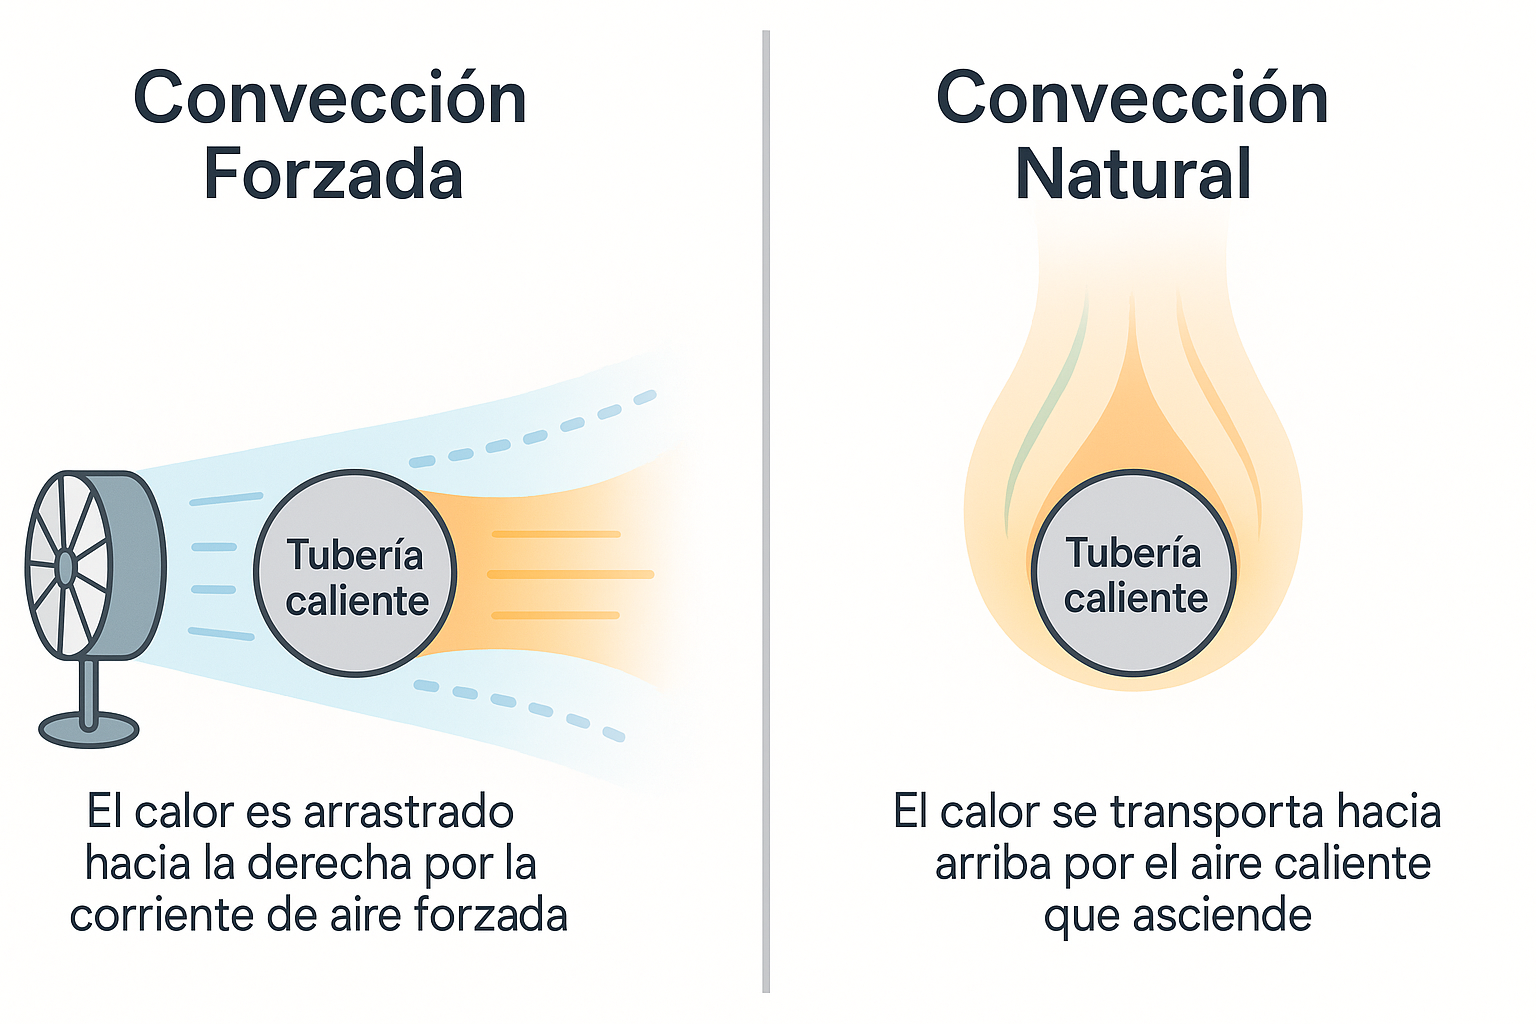
\includegraphics[width=0.6\textwidth]{figures/cap1/natural_forzada.png}
    \label{fig:natural_forzada} 
 \caption{Comparación esquemática de la transferencia de calor alrededor de una tubería caliente: (izquierda) convección forzada; (derecha) convección natural.} 
 \label{fig:natural_forzada}
\end{figure}


Los primeros estudios sobre la transferencia de calor por convección trataron las ramas de la convección forzada y la convección natural de forma separada, sin considerar la posible interacción entre ambas. Por un lado, los experimentos de Henri Bénard (1901) marcaron un hito en la comprensión de la convección natural \cite{benard1901}. Más tarde, Lord Rayleigh (1916) desarrolló la base teórica de la inestabilidad térmica en capas fluidas \cite{rayleigh1916}. En paralelo, en el ámbito de la convección forzada, trabajos como el de Dittus y Boelter (1930) establecieron correlaciones empíricas para la transferencia de calor en tubos \cite{dittus1930}. No fue sino hasta mediados del siglo XX que comenzó a reconocerse que ambos mecanismos pueden coexistir en muchas configuraciones de interés práctico. Así surgió el concepto de convección mixta, donde la convección forzada y la natural actúan simultáneamente como casos extremos de un fenómeno más general \cite{tao1960,metais1964}. 

\subsection*{Régimen de Transición y Transición Laminar-Turbulenta}

Cuando un fluido se desplaza a través de un conducto o sobre una superficie, su movimiento puede clasificarse en dos tipos de régimen: laminar o turbulento. En el régimen laminar, el flujo es ordenado y las partículas del fluido se mueven en capas paralelas sin mezclarse entre sí. En cambio, en el régimen turbulento, el flujo es caótico, con remolinos, tiende a mezclarse, y presenta fluctuaciones en los campos de velocidad y presión. En ese sentido, un flujo que se encuentra en un estado desarrollado\footnote{Esto es, sus magnitudes no varían con el tiempo o con el espacio en un sentido estadístico.} intermedio, de transición , se dice que el flujo está en régimen de transición. Este estado de flujo no debe confundirse con la transición laminar-turbulenta del sistema, donde el flujo evoluciona de un régimen laminar a un régimen turbulento completamente desarrollado. Esta transición puede ocurrir en el tiempo (transición laminar-turbulenta temporal) o en el espacio (transición laminar-turbulenta espacial).

Por otro lado, la transición laminar-turbulenta es un fenómeno de gran importancia para la ingeniería y la física aplicada ya que está presente en diferentes dispositivos termohidráulicos. El cambio de un régimen a otro puede tener un impacto significativo en la transferencia de calor, especialmente en aplicaciones de convección mixta. El coeficiente de fricción (factor de Darcy) o el coeficiente de convección (numéro de Nusselt) se incrementan notablemente cuando se produce la transición \cite{incropera,white}. En ese sentido, este estado no es deseado desde el punto de vista ingenieril ya que es intermitente (es decir, el flujo puede fluctuar entre los regímenes laminar y turbulento), sin embargo, el estudio de la transición es relevante para poder controlar el fenómeno o anticipar, y por tanto aprovechar, su comportamiento. Por ejemplo, un problema importante se da en el diseño de intercambiadores de calor cuando el punto de trabajo del flujo dentro de los tubos o conductos se encuentra en régimen de transición donde las magnitudes relevantes (como coeficientes de fricción y de transferencia de calor) tienen una gran variación \cite{ghajar2019heat}.

La evolución de un flujo, tanto en el tiempo como en el espacio, depende de las perturbaciones externas que reciba (por ejemplo, cambios de presión o de temperatura), de las condiciones de borde a las que esté sometido (como puede ser la rugosidad, flujo de calor en las paredes o gradientes de presión, entre otros) y de la respuesta del propio sistema, determinada por sus propiedades físicas y el régimen de flujo. Para modelar matemáticamente las condiciones que pueden modificar ese régimen —es decir, los estados iniciales capaces de desencadenar una transición— y analizar cómo dicha transición impacta en la transferencia de calor, se recurre a la teoría de estabilidad hidrodinámica. Esta teoría ofrece un marco para predecir cuándo un flujo laminar se volverá inestable mediante el estudio de la evolución de pequeñas perturbaciones: si estas crecen en el espacio o en el tiempo, el flujo pierde su estabilidad y eventualmente transiciona hacia un régimen turbulento.

La investigación teórica sobre la transición ha tenido un desarrollo histórico notable que se remonta al siglo XIX, con el célebre experimento de Osborne Reynolds \cite{reynolds1883}, que marcó el inicio del estudio sistemático del fenómeno. A comienzos del siglo XX, Orr \cite{orr1907} y Sommerfeld \cite{sommerfeld1908} formalizaron las bases de la estabilidad hidrodinámica al desarrollar las ecuaciones linealizadas que llevan sus nombres, conocidas como ecuaciones de Orr-Sommerfeld. Estas describen la evolución de perturbaciones en un flujo y son fundamentales para comprender los mecanismos de transición. Un avance crucial se produjo con los trabajos de Tollmien \cite{tollmien1930} y Schlichting \cite{schlichting1933}, quienes describieron de forma teórica el estado lineal de la transición; esta teoría fue confirmada experimentalmente en el estudio de la capa límite sobre una placa plana realizado por Schubauer y Skramstad \cite{schubauer1947laminar}. Finalmente, la incorporación de la teoría de inestabilidad secundaria por Herbert \cite{herbert1983secondary} permitió extender el análisis al caso tridimensional, ofreciendo así una comprensión más completa del fenómeno.


\section{Motivación}

En la actualidad, muchos problemas de ingeniería presentan flujos en régimen de transición. La mayoría de los flujos en estás condiciones son no isotérmicos \cite{chen2003direct}. El estudio de la transferencia de calor en la transición laminar-turbulenta es importante en diversas aplicaciones ingenieriles, como en los elementos combustibles de reactores nucleares, en intercambiadores de calor, en los álabes de una turbina, equipos electrónicos, entre otros.

Por otro lado, el fenómeno de convección mixta puede manifestarse conjuntamente en flujos atmosféricos \cite{pirozzoli2017mixed} como también en aplicaciones de ingeniería presentes en el proceso de fabricación de silicio, la refrigeración de equipos electrónicos, paneles solares térmicos, álabes de turbinas, intercambiadores de calor de diverso tipo, reactores nucleares, entre otros \cite{kasagi1997direct}. 

Entre las aplicaciones técnicas de mayor relevancia de la convección mixta se destaca el transporte de energía térmica. En las últimas décadas se han realizado muchos esfuerzos para desarrollar técnicas tendientes a mejorar la transferencia de calor y el desempeño global de los intercambiadores de calor. El interés en estas técnicas radica en el ahorro de la energía. En este sentido, las necesidades energéticas actuales propician el diseño y la mejora constante de los reactores nucleares utilizados para la provisión de energía eléctrica. Dentro de la nueva generación de reactores nucleares GEN-IV\footnote{\url{https://www.gen-4.org/}}, de los seis conceptos especificados, uno corresponde a reactores tipo GFR (\textit{Gas-cooled Fast Reactor}) que utiliza como refrigerante gas helio cuyo número de Prandtl es Pr$\simeq0.7$ similar al aire.


\section{Objetivos}

El objetivo del presente trabajo es el estudio de la transferencia de calor en régimen de transición laminar-turbulenta en convección mixta. Para ello se emplea la herramienta numérica Incompact3D. Se obtienen resultados numéricos para números de Reynolds entre $2000$ y $5000$, números de Prandt igual a $0.071$ y $0.71$ y numéros de Richardson entre $0.04$ y $106$.

Parte de las tareas secundarias para la realización de trabajo incluyeron:

\begin{itemize}

	\item Entrenamiento y manejo en el uso de la herramienta numérica Incompact3D.
	
	\item Validación de la herramienta numérica y simulación de flujos turbulentos.

	\item Validación de l de métodos para inestabilizar soluciones laminares en la herramienta
numérica.

\end{itemize}

\textcolor{red}{No se como escribir esta parte. Como escribir el uso y validación de la herramienta de Szuban y todo lo demas que queda referido a los objetivos.}





\section{Organización del trabajo}
\chapter{Modelo Matemático} \label{cap:modelo}

En este capítulo se presenta el marco teórico que sustenta este trabajo. Se introduce brevemente el concepto de turbulencia y de simulaciones DNS. Luego, se describen las ecuaciones, junto con las condiciones de borde, empleadas para modelar el sistema físico bajo análisis: un canal de placas paralelas sometido a un flujo de calor constante en las paredes. Asimismo, se definen las magnitudes estadísticas necesarias para el tratamiento de los datos obtenidos mediante simulaciones.

Por otra parte, se incluye un breve resumen del análisis de estabilidad lineal que constituye la base teórica para el cálculo numérico de los autovalores y autofunciones empleados en la construcción de las perturbaciones utilizadas para inestabilizar flujos con convección mixta. Estas perturbaciones se aplican en el Capítulo \ref{cap:transicion}, donde se analiza la transición temporal laminar–turbulenta.

\section{El concepto de turbulencia. Simulaciones Numéricas Directas (DNS)}

Los flujos se clasifican, de manera general, en laminares, de transición y turbulentos. La mayoría de los flujos presentes en la naturaleza y en aplicaciones industriales son turbulentos, por lo que su estudio tiene un gran interés tanto en el ámbito científico como en el tecnológico. Algunos ejemplos de flujo turbulento se encuentran presentes en el movimiento de las nubes en el cielo, las corrientes oceánicas, el flujo sobre el ala de un avión o el flujo sobre el álabe de una turbina, entre muchos otros.

Todos estos flujos presentan un comportamiento aparentemente aleatorio y caótico, lo cual se refleja en las variaciones espaciales y temporales de las variables del flujo, tales como la velocidad, la temperatura o la densidad. Las complejidades inherentes a la turbulencia dificultan su definición de forma concisa; por ello, en general, no es común dar una definición de turbulencia sino más bien presentar ciertos atributos canónicos \cite{smits2009lectures}:

\begin{itemize}
	
	\item \textbf{Tridimensionalidad.} La turbulencia es un fenómeno inherentemente tridimensional. 
	
	\item \textbf{Naturaleza no estacionaria.} Los flujos turbulentos evolucionan en el tiempo y se caracterizan por variaciones inestables en magnitudes asociadas (velocidad, presión, temperatura, etc).
	
	\item \textbf{Carácter multiescala.} La turbulencia involucra una amplia gama de escalas en el espacio y en el tiempo. 
	
	\item \textbf{Difusividad.} Se tiene una mezcla eficaz\footnote{El término ``mezcla eficaz'' se refiere a la capacidad de un flujo turbulento para mezclar y dispersar las diferentes propiedades del fluido de manera rápida y homogénea.} de todas las propiedades del fluido (masa, velocidad, temperatura, concentración, etc.).

\end{itemize}

Por su relevancia práctica y su naturaleza aleatoria y compleja, este fenómeno ha sido objeto de un gran número de investigaciones teóricas y experimentales a lo largo de los últimos dos siglos. Incluso en la actualidad, se sigue estudiando con el objetivo de entender mejor su complejidad. En este contexto, el uso de la computación para resolver las ecuaciones que gobiernan la dinámica de fluidos ha adquirido un papel preponderante y se ha consolidado como una de las herramientas más utilizadas para el análisis de flujos turbulentos.

El rápido progreso de las computadoras de alto rendimiento, permite que la simulación numérica directa (\textit{Direct Numerical Simulation}, DNS) sea una herramienta fundamental para la investigación de la turbulencia \cite{moin1998direct}. Esta permite calcular la solución tridimensional y no estacionaria de las ecuaciones de conservación involucradas. Al resolverse sin recurrir a modelos de turbulencia, estas simulaciones requieren una precisión elevada para capturar todas las escalas del flujo \cite{pope2001turbulent}.

\section{Descripción del sistema bajo estudio. Ecuaciones de Gobierno}

Se considera el sistema representado en la Figura \ref{fig:sistem_domain} donde la dinámica de un fluido viscoso e incompresible sucede entre dos paredes paralelas e infinitas ubicadas en $y=\pm d$. Esto constituye un canal vertical de placas paralelas donde ambas paredes están sometidas a un flujo de calor constante $q''_w$.

\begin{figure}[H]
 \centering
  \subfloat[]{
    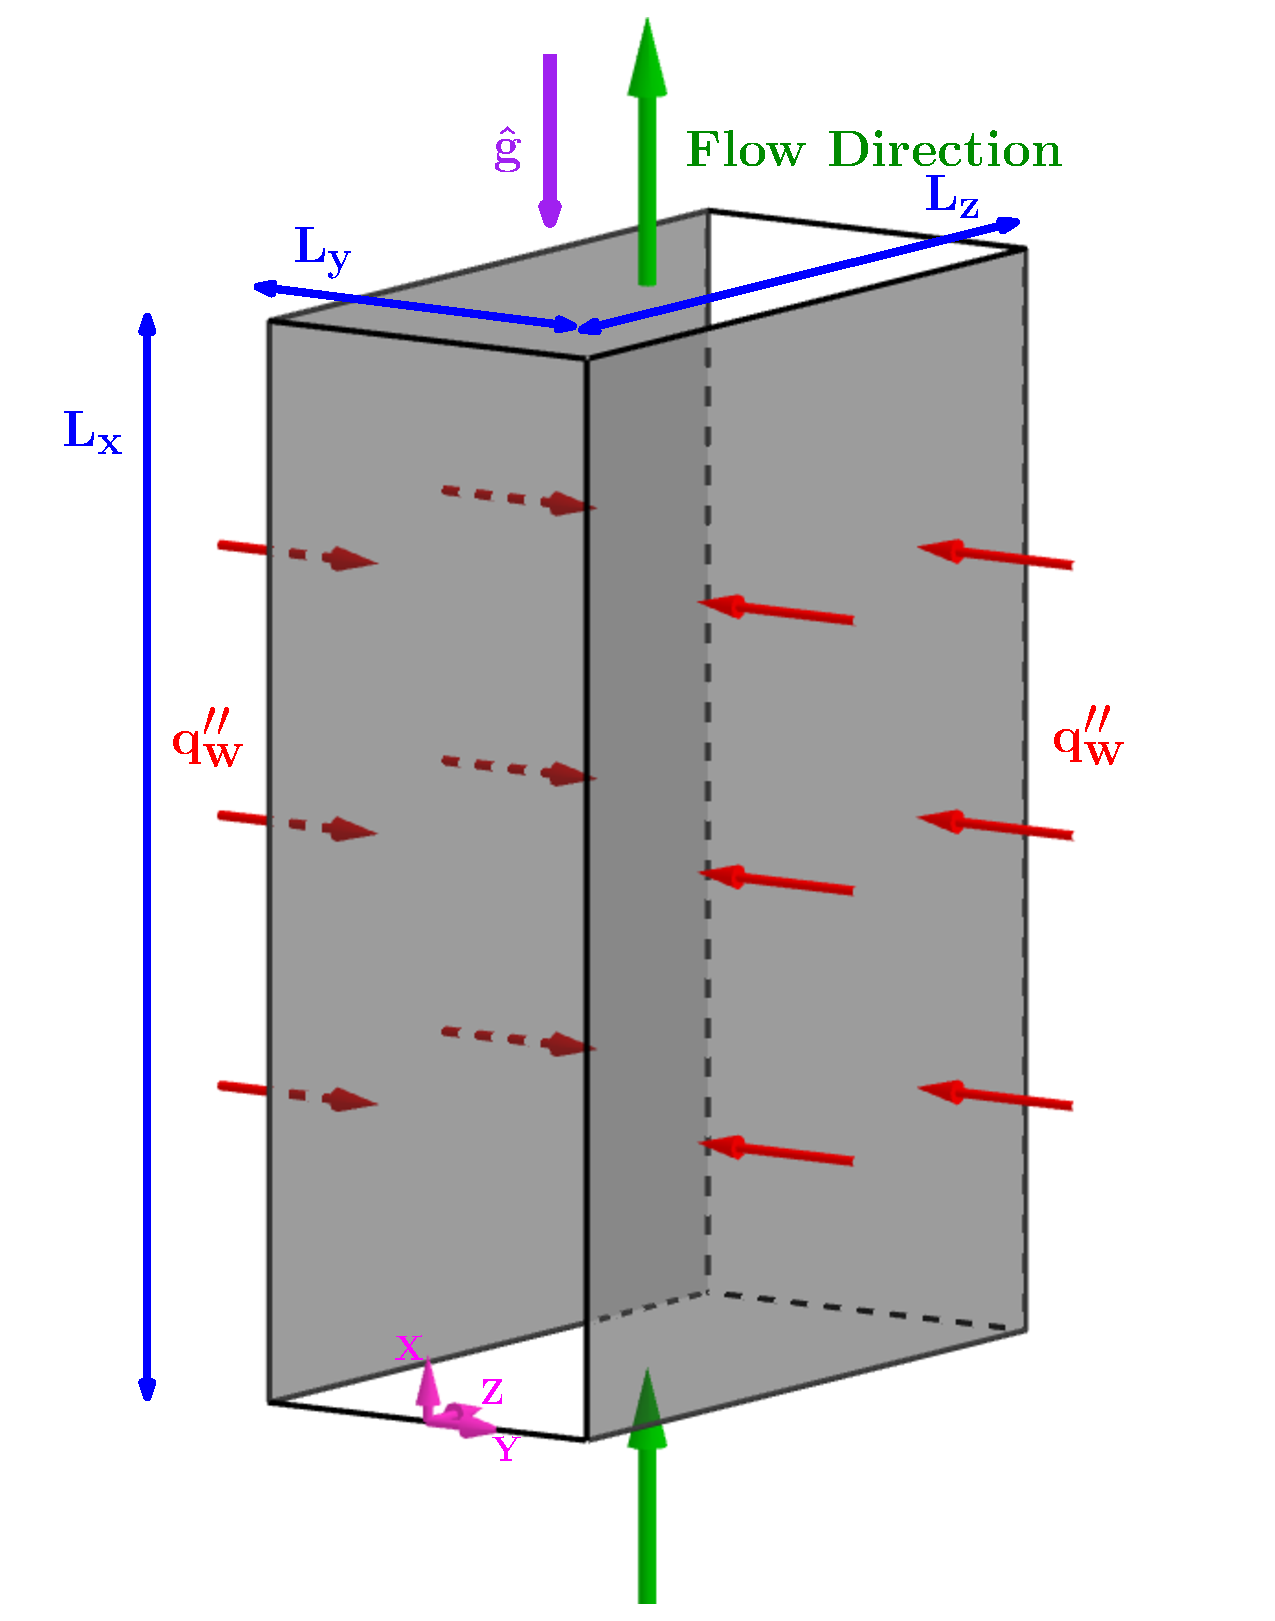
\includegraphics[width=0.49\textwidth]{figures/cap2/domain3d.eps}
    \label{fig:dom3d}}  
    \subfloat[]{
    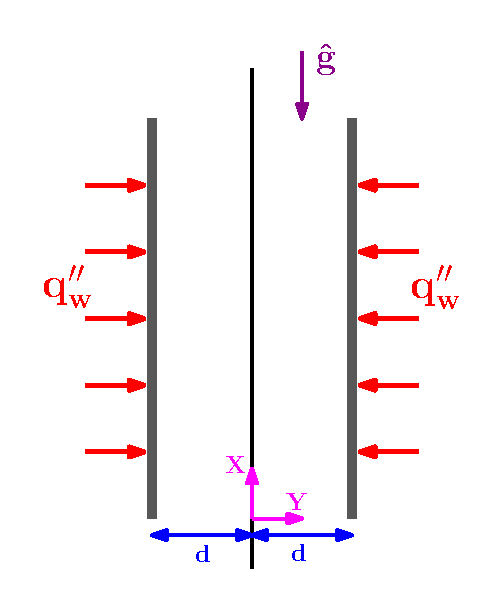
\includegraphics[width=0.49\textwidth]{figures/cap2/domain2d.eps}
    \label{fig:dom2d}}  
 \caption{Esquema del sistema físico bajo análisis.} 
 \label{fig:sistem_domain}
\end{figure}

El flujo ocurre en la dirección de la corriente (\textit{streamwise}) paralelo al eje X y su sentido es opuesto a la aceleración de la gravedad. Esta configuración se conoce como flujo ascendente o \textit{aiding flow}. Las ecuaciones de gobierno corresponden a los principios de conservación de masa, momento y energía que se expresan en el cuadro \ref{eq:gob_system}.

\begin{equation}
        \boxed{ \begin{array}{lcc}
			  %\\
              &  \nabla \cdot \left( \rho_o \mathbf{u} \right) = 0 \\
              \vspace*{2mm}
              &  \frac{\partial \left( \rho_o \mathbf{u} \right)}{\partial t} + \mathbf{u} \cdot \nabla  \left( \rho_o \mathbf{u} \right) = -\nabla \text{p} + \mu_o \hspace{1mm} {\nabla}^2 \mathbf{u}  + \rho(T) \hspace{1mm} \mathbf{g} \\
              \vspace*{2mm}
              &  \frac{\partial T}{\partial t} + \mathbf{u} \cdot \nabla T =  \alpha \hspace{1mm} \nabla^2 T  \\
              % \\
             \end{array}
               }
             \label{eq:gob_system}
\end{equation}

Un sistema físico cuyas dimensiones ``son muy grandes'' (o infinitas) constituye un sistema ideal. En él, es posible ubicar el origen de nuestro sistema de referencia lejos de los extremos a fin de evitar efectos de bordes. Allí, el flujo se encuentra completamente desarrollado y ha alcanzado un estado estadísticamente estacionario, es decir, sus valores estadísticos, como el promedio o la varianza, no varían en el tiempo. En este contexto, la condición de flujo de calor constante en las paredes se imponen como condiciones de Neumann:

\begin{equation}
\kappa \hspace{0.5mm} \left. \frac{\partial T}{\partial y} \right\vert_{y=\mp d} = \pm q''_w \text{.}
\label{eq:neumann}
\end{equation}

Debido a una limitación computacional evidente, nuestro modelo no puede abarcar dicha extensión. En ese sentido, el ``dominio infinito'' se reemplaza con un dominio acotado de dimensiones $L_x \times L_y \times L_z$ (Figura \ref{fig:dom3d}) adoptando condiciones de borde periódicas (PBC) en la direcciones $X$ y $Z$:
\begin{align}
\xi(x=0,y,z,t) &= \xi(x=L_x,y,z,t)
\label{eq:pbc1} \\
\xi(x,y,z=0,t) &= \xi(x,y,z=L_z,t)
\label{eq:pbc2}
\end{align}
siendo $\xi$ un campo escalar arbitrario. Esto se puede interpretar como si las PBC crearan ``la ilusión'' de un dominio infinito, mediante la repetición de este dominio finito en el espacio.

Por otra parte, como se ha mencionado, dado que un flujo turbulento no es estacionario, aparecen fluctuaciones del flujo de calor y de la temperatura sobre la superficie de la pared. En este contexto, algunos autores \cite{kasagi1992direct,tao1960} asumen que dichas fluctuaciones son pequeñas a fin de considerar que la temperatura en la pared es localmente isotérmica y que además, el flujo de calor no varía en la dirección de la corriente. Eso equivale a suponer que la temperatura en la pared, promediada en el tiempo y en la dirección $Z$, crece linealmente con la coordenada $x$, y por lo tanto: 

$$
\langle T_w \rangle = \mathcal{A} \hspace{0.5mm} x.
$$

Debido al crecimiento lineal de $\langle T_w \rangle$, es requerido realizar el cambio de variable $T(x,y,z,t) = \langle T_w \rangle - \theta(x,y,z,t)$ para que sigan siendo válidas las condiciones de borde periódicas (ecuaciones \ref{eq:pbc1} y \ref{eq:pbc1}). Dicha modificación introduce un término fuente en la ecuación de conservación de energía:

\begin{equation}
\frac{ \partial \theta }{ \partial t } + \mathbf{u} \cdot \nabla \theta = \alpha \nabla^2 \theta + \mathcal{A} \hspace{0.5mm} u_x 
\label{eq:energy_pcb_source}
\end{equation}

Asimismo, se emplea la aproximación de Bousinessq que supone que los cambios de densidad en el fluido pueden despreciarse, excepto donde la densidad está multiplicada por $\mathbf{g}$ \cite{kundu}. El término $\rho(T) \mathbf{g}$ de la ecuación de momento se reescribe según la expresión \ref{eq:bussinesq}, donde $\rho_o \equiv \rho(T_R)$ y $\rho_w \equiv \rho(T=\langle T_w \rangle)$ \cite{incropera}. Luego, la ecuación de momento queda reescrita como se expresa en la ecuación \ref{eq:mom_rewrite} siendo $\mathbf{\hat{e_g}}=(-1,0,0)$, $\rho_{w/2} \equiv \rho(T=\langle T_w \rangle / 2)$ y $C$ es una constante que no depende de $x$.

\begin{equation}
\begin{aligned}
\rho(T) \mathbf{g} &= \rho_o \left[ 1 - \beta (T - T_R) \right] \mathbf{g} \\
				   &= \rho_o \left[ 1 - \beta ( \hspace{0.5mm} (\langle T_w \rangle - \theta) - T_R) \right] \mathbf{g} \\
 		           &= \rho_o \beta \theta \mathbf{g} + \rho_w \mathbf{g}
\end{aligned}
\label{eq:bussinesq}
\end{equation}

\begin{equation}
\frac{ \rho_o \hspace{0.5mm} \partial \mathbf{u}}{\partial t} + \mathbf{u} \cdot \nabla  \left( \rho_o \mathbf{u} \right) = -\nabla \left[ \text{p} + \rho_{w/2} \hspace{0.5mm} g \hspace{0.5mm} x + C \right] + \mu_o \hspace{1mm} {\nabla}^2 \mathbf{u}  + g \hspace{0.5mm} \rho_o \hspace{0.5mm} \beta \hspace{0.5mm} \theta \hspace{0.5mm} \mathbf{\widehat{e_g}},
\label{eq:mom_rewrite}  
\end{equation}
%\rho_w \hspace{0.5mm} g \hspace{0.5mm} \mathbf{\widehat{e_g}}
 

Mediante el balance de energía en el volumen de control $L_x \times L_y \times L_z$, es posible demostrar que $\mathcal{A} = \frac{q''_w}{\rho_o  c_p U_b d}$ siendo $d$ el semiancho del canal y $U_b$ la velocidad \textit{bulk} \cite{pope2001turbulent}. Luego, empleando la velocidad en el centro del canal $U_o$, el semiancho $d$, la temperatura $T_o = \mathcal{A} \hspace{0.3mm} d $ y tomado $\text{p}^* = \left[ \text{p} + \rho_{w/2} \hspace{0.5mm} g \hspace{0.5mm} x + C \right] / \rho_o (U_o)^2$, el sistema de ecuaciones dimensional \ref{eq:gob_system} queda escrito en su forma adimensional como se muestra en el cuadro \ref{eq:gob_system_adim}. Los números adimensionales asociados a estas ecuaciones, se expresan en las relaciones \ref{eq:num_adim}, de izquierda a derecha, se tiene: el número de Reynolds, el número de Prandtl, el parámetro que acompaña al término boyante y al número de Richardson basado en el flujo de calor. 

Otro detalle importante es el hecho de que el fluido de trabajo es impulsado por un caudal másico constante. Esta cuestión se encuentra representada por el término fuente $f \hspace{0.3mm} \mathbf{\widehat{e_x}}$, en la ecuación de momento, donde $f$ es una constante en el espacio y varía con el tiempo de manera que mantiene constante el caudal total. 

\begin{equation}
\boxed{
\begin{array}{l}
    \nabla^* \cdot \mathbf{u^*} = 0 \\
    \frac{\partial \mathbf{u^*}}{\partial t^*} + \mathbf{u^*} \cdot \nabla^* \mathbf{u^*} = 
    -\nabla \text{p}^* + \frac{1}{\text{Re}_o} \hspace{0.5mm} \nabla^{*2} \mathbf{u^*} + \Pi \hspace{0.5mm} \theta^* \hspace{0.5mm} \mathbf{\widehat{e_g}} + f \mathbf{\widehat{e_x}}  \\
    \frac{\partial \theta^*}{\partial t^*} + \mathbf{u^*} \cdot \nabla^* \theta^* = 
    \frac{1}{\text{Re}_o \hspace{0.5mm} \text{Pr}} \hspace{0.5mm} \nabla^{*2} \theta^* + u_x^* 
\end{array}
}
\label{eq:gob_system_adim}
\end{equation}

\begin{equation}
\text{Re}_o = \frac{\mu_o}{\rho_o \hspace{0.5mm} U_o \hspace{0.5mm} d } \quad ; \quad \text{Pr}= \frac{\mu_o}{\rho_o \hspace{0.5mm} \alpha} \quad ; \quad \Pi = \frac{\text{Ri}_o}{\text{Re}_o \hspace{0.5mm} \text{Pr}} \quad ; \quad \text{Ri}_o = \frac{g \hspace{0.5mm} \beta \hspace{0.5mm} q''_w \hspace{0.5mm} d^2}{k \hspace{0.5mm} U_o^2}
\label{eq:num_adim}
\end{equation}
%siendo Ra, el número de Rayleigh.

Las condiciones de flujo de calor constante en las paredes se expresean, en su forma adimensional, en la ecuación \ref{eq:neumann_adim}. Sin embargo, estas condiciones pueden ser aproximadas como condiciones de Dirichlet ya que al suponer que la temperatura de las paredes es constante (fluctuaciones de temperatura despreciables) se obtiene: 
$$T(x,y=-d,z,t) = T(x,y=+d,z,t) = \langle T_w \rangle$$ 
Éste tipo de aproximación se conoce en la literatura como \textit{Mixed Boundary Condition} \cite{straub2019influence} y su forma adimensional se expresa en la ecuación \ref{eq:dirichlet_adim_theta}. Por último, para las componentes de la velocidad y del campo de presión, se adoptan condiciones de no deslizamiento y condiciones de Neumann homogéneas, respectivamente, en las paredes. 

\begin{align}
\begin{array}{l}
    \left. \frac{\partial \theta^*}{\partial y^*} \right\vert_{y^*=-1} = + \frac{2}{3} \text{Re}_o \hspace{0.5mm} \text{Pr} \\
    \left. \frac{\partial \theta^*}{\partial y^*} \right\vert_{y^*=+1} = - \frac{2}{3} \text{Re}_o \hspace{0.5mm} \text{Pr} 
\end{array}
\label{eq:neumann_adim}
\end{align}

\begin{equation}
\theta^*(x^*,y^*=0,z^*,t^*) = \theta^*(x^*,y^*=2,z^*,t^*) = 0
\label{eq:dirichlet_adim_theta}
\end{equation}



\subsection{Sumario de Ecuaciones}

\textbf{Ecuaciones de Gobierno:}
\begin{equation}
\begin{array}{l}
    \nabla^* \cdot \mathbf{u^*} = 0 \\
    \frac{\partial \mathbf{u^*}}{\partial t^*} + \mathbf{u^*} \cdot \nabla^* \mathbf{u^*} = 
    -\nabla \text{p}^* + \frac{1}{\text{Re}_o} \hspace{0.5mm} \nabla^{*2} \mathbf{u^*} + \frac{\text{Ri}_o}{\text{Re}_o \hspace{0.5mm} \text{Pr}} \hspace{0.5mm} \theta^* \hspace{0.5mm} \mathbf{\hat{g}} + f \mathbf{\widehat{e_x}}  \\
    \frac{\partial \theta^*}{\partial t^*} + \mathbf{u^*} \cdot \nabla^* \theta^* = 
    \frac{1}{\text{Pr}}\hspace{0.5mm}  \frac{1}{\text{Re}_o} \hspace{0.5mm} \nabla^{*2} \theta^* + u_x^* 
\end{array}
\label{eq:gob_system_res1}
\end{equation}

\textbf{Condiciones de borde:} considerando $\xi= u^*_x, u^*_y, u^*_z, \text{p}^*, \theta^*$, entonces
\begin{align}
&\xi(x^*=0,y^*,z^*,t^*) = \xi(x^*=L_x/d,y^*,z^*,t^*) 
	\label{eq:bc_1} \\
&\xi(x^*,y^*,z^*=0,t^*) = \xi(x^*,y^*,z^*=L_z/d,t^*) 
	\label{eq:bc_2} \\
&\theta^*(x^*,y^*=-1,z^*,t^*)       = \theta^*(x^*,y^*=+1,z^*,t^*) = 0
	\label{eq:bc_3} \\
&\mathbf{u^*}(x^*,y^*=-1,z^*,t^*)   = \mathbf{u^*}(x^*,y^*=+1,z^*,t^*) = 0
	\label{eq:bc_4} \\
&\partial_y \text{p}^*(x^*,y^*=-1,z^*,t^*) = \partial_y \text{p}^*(x^*,y^*=+1,z^*,t^*) = 0
	\label{eq:bc_5}
\end{align}

A lo largo de este trabajo, particularmente para el análisis de estabilidad lineal, se utiliza también la forma adimensional de las ecuaciones del trabajo de Chen \cite{chen1996linear} que se obtienen empleando el  semiancho del canal $d$, la velocidad \textit{bulk} $U_b$ y la temperatura $T_c = \text{Re} \hspace{0.5mm} \text{Pr} \hspace{0.5mm} \mathcal{A} \hspace{0.5mm} d$. Dichas ecuaciones se expresan en \ref{eq:gob_system_res2}. Las condiciones de borde son exactamente análogas a su forma adimensional de más arriba. Adicionalmente, aparece otro número adimensional conocido: el número de Rayleigh (Ra) basado en el flujo de calor y definido en la ecuación \ref{eq:Rayleigh}.

\begin{equation}
\begin{array}{l}
    \nabla^* \cdot \mathbf{v^*} = 0 \\
    \frac{\partial \mathbf{v^*}}{\partial t^*} + \mathbf{v^*} \cdot \nabla^* \mathbf{v^*} = 
    -\nabla \text{p}^* + \frac{1}{\text{Re}_b} \hspace{0.5mm} \nabla^{*2} \mathbf{u^*} + \frac{\text{Ra}}{\text{Re}_b} \hspace{0.5mm} \varphi^* \hspace{0.5mm} \mathbf{\hat{g}} + f \mathbf{\hat{x}} \\
    \frac{\partial \varphi^*}{\partial t^*} + \mathbf{v^*} \cdot \nabla^* \varphi^* = 
    \frac{1}{\text{Pr}}\hspace{0.5mm}  \frac{1}{\text{Re}_b} \hspace{0.5mm} \left[ \nabla^{*2} \varphi^* - v_x^* \right]  
\end{array}
\label{eq:gob_system_res2}
\end{equation}

\begin{equation*}
\varphi^* = -  \frac{\theta^*}{\text{Re}_o \hspace{0.5mm} \text{Pr}}  \quad ; \quad \mathbf{v^*} = \frac{2}{3} \mathbf{u^*} \quad ; \quad \text{Re}_b = \frac{2}{3} \text{Re}_o
\end{equation*}  

\begin{equation}
\text{Ra} = \frac{g \hspace{0.5mm} \beta \hspace{0.5mm} q''_w \hspace{0.5mm} d^3}{c_p \hspace{0.5mm} \alpha \hspace{0.5mm} \mu_o \hspace{0.5mm} U_b}
\label{eq:Rayleigh}
\end{equation} 


\section{Magnitudes estadísticas de flujos turbulentos} \label{sec:mag-stat}

En flujos turbulentos, los campos como la velocidad son variables aleatorias \\ \cite{pope2001turbulent}. Supóngase que $\xi$ es un campo arbitrario asociado al sistema. Para una posición e instante determinados en un experimento (o simulación) repetible bajo las mismas condiciones, y sin dependencia entre repeticiones, el conjunto $\lbrace \xi^{(1)}, \xi^{(2)}, \cdots \rbrace$ puede considerarse de variables i.i.d. (independientes e idénticamente distribuidas). Entonces, el promedio en ensemble sobre $N$ repeticiones se define como 

\begin{equation*}
\langle \xi \rangle_N = \frac{1}{N} \sum^N_{n=1} \xi^{(n)} 
\end{equation*}
siendo $N$ muy grande. Si el sistema es estadísticamente estacionario, sus propiedades estadísticas no cambian con el tiempo; si es estadísticamente homogéneo, no varían con la posición; y si es ergódico \cite{moser2003}, el promedio en ensemble puede reemplazarse por el promedio en el tiempo y/o en el espacio (direcciones homogéneas). 

En problemas de turbulencia, los promedios y las fluctuaciones de las variables de interés son importantes, por lo que la descomposición de Reynolds \cite{pope2001turbulent, kundu} de la variable instantánea arbitraria $\xi$ puede representarse como un valor promedio $\langle \xi \rangle$ y una fluctuación $\xi^{\prime}$:

$$\xi = \langle \xi \rangle + \xi^{\prime}$$
donde $\langle (\text{.}) \rangle$ denota el promedio estadístico y $(\text{.})^{\prime}$ denota la parte fluctuante. 

Supongase entonces, que $\eta$ es otra magnitud instantánea del flujo. El promedio de la multiplicación  de las fluctuaciones de $\xi$ y $\eta$ son cantidades de interés para la construcción de modelos de turbulencia \cite{pope2001turbulent}. Dichas cantidades nos indican que tan correlacionadas están $\xi$ y $\eta$ entre sí. Estas se obtienen a partir del promedio de las magnitudes totales, ecuación \ref{eq:mag-cov}, donde se usa el hecho de que el promedio de una fluctuación es nulo y el promedio de otro promedio sigue siendo él mismo \cite{pope2001turbulent}. De esta manera, el promedio del producto de fluctuaciones $\langle \xi^{\prime} \eta^{\prime} \rangle$ queda expresado en la ecuación \ref{eq:fluct-corr}.

\begin{equation}
\begin{aligned}
\langle \xi \eta \rangle &= \langle (\langle \xi \rangle + \xi^{\prime}) (\langle \eta \rangle + \eta^{\prime}) \rangle \\
                         &= \langle \xi \rangle \langle \eta \rangle + \langle \xi^{\prime} \eta^{\prime} \rangle
\end{aligned}
\label{eq:mag-cov}
\end{equation}

\begin{equation}
\langle \xi^{\prime} \eta^{\prime} \rangle = \langle \xi \eta \rangle - \langle \xi \rangle \langle \eta \rangle
\label{eq:fluct-corr}
\end{equation}

Algunas cantidades importante que aparecen en las ecuaciones promediadas de conservación (ecuaciones RANS \cite{kundu}) son:

\begin{itemize}
	\item $\langle u^{\prime}_i u^{\prime}_j \rangle$: componentes del tensor de Reynolds con $i,j=x,y,z$;
	\item $\langle \theta^{\prime} u^{\prime}_i \rangle$: flujos turbulentos de calor en la dirección $i$, con $i=x,y,z$;
	\item $\langle \theta^{\prime} \theta^{\prime} \rangle$: varianza de la temperatura;

	\item otra magnitud utilizada ampliamente a lo largo de este trabajo es la energía cinética turbulenta $k$ (o TKE) definida como proporcional a la traza del tensor de Reynolds, esto es, 

\begin{equation}
k = \frac{1}{2} \left[ \langle u^{\prime}_x u^{\prime}_x \rangle + \langle u^{\prime}_y u^{\prime}_y \rangle + \langle u^{\prime}_z u^{\prime}_z \rangle \right] \text{.}
\label{eq:tke}
\end{equation}

\end{itemize}


\section{Teoría de Estabilidad Lineal. Perturbaciones} \label{line_an}

La evolución de un flujo laminar a uno turbulento (transición laminar-turbulenta) es crucial en ingeniería ya que las características del mismo varían notablemente entre estos regímenes. Por ejemplo, los coeficientes de fricción y de convección aumentan considerablemente al pasar de un régimen laminar a uno turbulento \cite{machaca2024}. Las ecuaciones de Navier–Stokes admiten ambas soluciones bajo ciertos requisitos, lo que implica que el tipo de flujo y su evolución dependen de las perturbaciones y las condiciones impuestas sobre el sistema. 

Para analizar la estabilidad lineal y prever de forma matemática cómo cambiará el flujo una vez perturbado, resulta indispensable conocer el flujo base sobre el que se añaden las perturbaciones para desencadenar las inestabilidades que dan paso a la transición. En este trabajo se adopta como flujo base al flujo laminar completamente desarrollado. %En consecuencia, la evolución de las perturbaciones también queda condicionada por dicho estado inicial. 



\subsection{Flujo Base}

Si el flujo está completamente desarrollado, tanto térmica como hidrodinámicamente, entonces el mismo sólo dependerá de la variable $y^*$. El sistema de ecuaciones \ref{eq:gob_system_res2} puede reducirse a la ecuación de momento en la dirección $X$ y a la ecuación de energía \cite{chen1996linear}, las cuales quedan expresadas de la forma 

\begin{align}
&\frac{d \text{p}^* }{d x^*} = \frac{\text{Ra}}{\text{Re}_b } \Phi^* + \frac{1}{\text{Re}} \frac{d^2 V^*_x}{d {y^*}^2}, \\
&\frac{d^2 \Phi^*}{ d {y^*}^2 } =  V^*_x \text{.}
\label{eq:base1}
\end{align}
El perfil de velocidad y de temperatura admiten las condiciones de borde \\  $V^*_x({y^*}= \pm 1) = \Phi^* ({y^*}= \pm 1) = 0 $. Las soluciones para un flujo asistido por fuerzas boyantes ($\text{Ra}>0$) están dadas por las expresiones \ref{eq:vel_asist_boyant} y \ref{eq:theta_asist_boyant}, mientras que para un flujo donde las fuerzas boyantes son opuestas ($\text{Ra}<0$), las soluciones quedan definidas por las ecuaciones \ref{eq:vel_opo_boyant} y \ref{eq:theta_opo_boyant} \cite{chen1996linear}. Obsérvese que el único parámetro relevante aquí es el número de Rayleigh.
\small{
\begin{equation}
V^*_x = \frac{-E}{\sqrt{\text{Ra}}} \frac{\sinh(\kappa(1+y^*))\sin(\kappa(1-y^*)) + \sinh(\kappa(1-y^*))\sin(\kappa(1+y^*)) }{\cosh(2\kappa) + \cos(2\kappa)}
\label{eq:vel_asist_boyant}
\end{equation}

\begin{equation}
\Phi^* = \frac{E}{\text{Ra}} \left[ 1 - \frac{\cosh(\kappa(1+y^*))\cos(\kappa(1-y^*)) + \cosh(\kappa(1-y^*))\cos(\kappa(1+y^*))}{\cosh(2\kappa) + \cos(2\kappa)} \right] 
\label{eq:theta_asist_boyant}
\end{equation}


\begin{equation}
V_x = \frac{F}{2 m^2} \left( \frac{\cosh(m y^*)}{\cosh(m)} - \frac{\cos(m y^*)}{\cos(m)} \right) 
\label{eq:vel_opo_boyant}
\end{equation}

\begin{equation}
\Phi^* = \frac{F}{2 m^4} \left( \frac{\cosh(m y^*)}{\cos(m)} + \frac{\cos(m y^*)}{\cos(m)} - 2 \right) 
\label{eq:theta_opo_boyant}
\end{equation}

\begin{equation*}
\kappa = \frac{\text{Ra}^{-1/4}}{\sqrt{2}} \quad ; \quad m = (-\text{Ra})^{1/4} \quad ; \quad F = \frac{2 m^3}{\tanh(m)-\tan(m)} \quad ; \quad
\end{equation*}

\begin{equation*}
E= -2 \kappa \hspace{1mm} \text{Ra}^{1/2} \hspace{1mm} \frac{\cosh(2\kappa) + \cos(2\kappa)}{\sinh(2\kappa) - \sin(2\kappa)} 
\end{equation*}
}

\subsection{Análisis de Estabilidad Lineal} \label{sec:estabilidad}

El análisis de estabilidad lineal permite evaluar cómo se comporta un flujo ante perturbaciones, identificando los mecanismos que pueden inducir transiciones o estados de intermitencia. En el caso de flujos de fluidos, condiciones como un número de Reynolds inferior a un valor crítico garantizan la estabilidad de un flujo laminar suave \cite{drazin2004hydrodynamic}. Sin embargo, en ocasiones, las perturbaciones crecen hasta alcanzar amplitudes finitas y establecer nuevos equilibrios estacionarios, que pueden volverse inestables a su vez y evolucionar hacia un régimen turbulento. Dos motivaciones principales para estudiar la estabilidad de los fluidos son: comprender el proceso de transición de un flujo laminar a uno turbulento, y predecir el inicio de dicha transición.

El enfoque parte de las ecuaciones de gobierno \ref{eq:gob_system_res2} donde se han omitido los superíndices ``*''. La idea consiste en suponer que los campos solución ($\mathbf{v}$, $\text{p}$, $\varphi$) pueden descomponerse como un flujo base más una perturbación:

\begin{align}
\mathbf{v} &= \mathbf{V} + \widetilde{\mathbf{v}} \\
\text{p} &= P + \widetilde{p} \\
\varphi &= \Phi + \widetilde{\varphi}
\end{align}  
donde las letras mayusculas hacen referencia al flujo base laminar y aquellas letras con $\widetilde{(\text{.})}$ a las perturbaciones. 

Despreciando términos de segundo orden, esto es, productos de perturbaciones, y asumiendo que los flujos bases son los flujos laminares desarrollados $\mathbf{V} = (V_x(y),0,0)$ y $\Phi \equiv \Phi(y)$ es posible expresar las ecuaciones que describen la dinámica de $\widetilde{\mathbf{v}}$, $\widetilde{p}$ y $\widetilde{\varphi}$ de la siguiente forma: 

\begin{align}
&\nabla \cdot \mathbf{\widetilde{v}} = 0
\label{eq:pertub_continuity} \\
&\partial_t \mathbf{\widetilde{v}} + V_x \hspace{1mm} \partial_x \mathbf{\widetilde{v}} + {\widetilde{v_y}} \partial_y V_x \hspace{1mm} \mathbf{\hat{e_x}} = - \nabla \widetilde{p} + \frac{1}{\text{Re}_b} \hspace{1mm} \nabla^2 \mathbf{\widetilde{v}} + \frac{\text{Ra}}{\text{Re}_b} \hspace{1mm} \widetilde{\varphi} \hspace{1mm}  \mathbf{\widehat{e_x}} 
\label{eq:pertub_momentum} \\
&\partial_t {\widetilde{\varphi}} + V_x \hspace{1mm} \partial_x {\widetilde{\varphi}} + {\widetilde{v_y}} \partial_y \Phi \hspace{1mm} = \frac{1}{\text{Re}_b \hspace{1mm} \text{Pr}} \left[ \nabla^2 \widetilde{\varphi} - \widetilde{v_x} \right]
\label{eq:pertub_energy} 
\end{align} 

Luego, aplicando el operador divergencia a la ecuación \ref{eq:pertub_momentum} es posible encontrar una expresión para el laplaciano de la presión:

\begin{equation}
- \nabla \widetilde{p} = 2 \hspace{1mm} \partial_x \widetilde{v_y} \hspace{1mm} \partial_y V_x - \frac{\text{Ra}}{\text{Re}_b} \partial_x \widetilde{\varphi}
\label{eq:pressure_eigen}
\end{equation}
Aplicando el operador laplaciano a la componente Y de la ecuación \ref{eq:pertub_momentum} es posible eliminar el término que involucra la presión, resultando en la siguiente expresión:

\begin{equation}
\left\lbrace \left[ \partial_t + V_x \partial_x \right] \nabla^2 - D^2(V_x) \partial_x - \frac{1}{\text{Re}_b} \nabla^4 \right\rbrace \widetilde{v_y} = - \frac{\text{Ra}}{\text{Re}_b} \hspace{1mm} \partial_{xy} \widetilde{\varphi}
\label{eq:eigensis_ec1}
\end{equation}
donde $D^j \equiv \partial^j_y$.

Para la descripción completa de las perturbaciones se utiliza la componente Y de la vorticidad $\widetilde{\eta} \equiv \partial_z \widetilde{v_x} - \partial_x \widetilde{v_z}$ cuya dinámica está dada por la ecuación \ref{eq:eigensis_ec2}.

\begin{equation}
 \left[ \partial_t + V_x \partial_x - \frac{1}{\text{Re}_b} \nabla^2  \right] \widetilde{\eta}  +  D(V_x) \hspace{1mm} \partial_z \widetilde{v_y} = \frac{\text{Ra}}{\text{Re}_b} \hspace{1mm} \partial_{z} \widetilde{\varphi}
\label{eq:eigensis_ec2}
\end{equation}

Así, las ecuaciones \ref{eq:pertub_energy}, \ref{eq:eigensis_ec1} y \ref{eq:eigensis_ec2} constituyen un sistema de EDP de 3 ecuaciones con 3 campos incognitas. A partir de los campos escalares $\widetilde{\eta}$ y $\widetilde{v_y}$, utilizando la ecuación \ref{eq:pertub_continuity} y la definición de $\widetilde{\eta}$ es posible hallar los campos $\widetilde{v_x}$ y $\widetilde{v_z}$. Asimismo, empleando la ecuación \ref{eq:pressure_eigen} y los campos $\widetilde{v_y}$ y  $\widetilde{\varphi}$ es posible hallar el campo de presión  $\widetilde{p}$. 

Las soluciones a dicho problema se proponen como ondas planas tridimensionales. Si $\widetilde{\xi}$ es una perturbación cualquiera, entonces, se escribe de la siguiente forma arbitraria:

\begin{equation}
\widetilde{\xi} = \hat{\xi}(y) \hspace{1mm} e^{i \left[ \alpha x + \beta z - \alpha c t \right]}
\label{eq:waves3d}
\end{equation}
donde $c \equiv c_r + i \hspace{0.5mm} c_i$ es la velocidad de fase y $\omega \equiv \alpha c$ es la frecuencia angular. Además: 

\begin{equation*}
\alpha \hspace{1mm}, \hspace{1mm} \beta \hspace{1mm} , \hspace{1mm} c_r \hspace{1mm} , \hspace{1mm} c_i \quad \epsilon \quad \mathbb{R}
\end{equation*}

En este sentido, dado que se busca y se estudia la transición temporal, se distinguen dos casos \cite{szuban2023}:

\begin{itemize}
\item[$\blacklozenge$] Si $\alpha c_i > 0$ entonces las perturbaciones crecen en el tiempo. El flujo se vuelve inestable.

\item[$\blacklozenge$] Si $\alpha c_i < 0$ entonces las perturbaciones decaen exponencialmente en el tiempo y la pertubación se atenúa. El flujo se vuelve estable.
\end{itemize}

Al reemplazar las soluciones tipo \ref{eq:waves3d} en el sistema de ecuaciones se obtiene un problema de autovalores generalizado de la siguiente forma:

\begin{equation}
\begin{bmatrix}
a_{11} & a_{12} & 0 \\[4pt]
a_{21} & a_{22} & a_{23} \\[4pt]
a_{31} & a_{32} & a_{33}
\end{bmatrix}
\,\begin{bmatrix}
\widehat{v_y} \\[4pt]
\widehat{\varphi} \\[4pt]
\widehat{\eta}
\end{bmatrix}
\;=\; i \omega
\,\begin{bmatrix}
  b_1 & 0 & 0 \\[4pt]
    0 & 1 & 0 \\[4pt]
    0 & 0 & 1
\end{bmatrix}
\,\begin{bmatrix}
\widehat{v_y} \\[4pt]
\widehat{\varphi} \\[4pt]
\widehat{\eta}
\end{bmatrix}
\label{eq:eigensistem-general}
\end{equation}

\begin{align*}
a_{11} &= \frac{1}{\text{Re}_b} \left[ D^2 - k^2 \right]^2 - i \alpha \left( V_x \left[ D^2 - k^2 \right] + D^2(V_x)\right) \hspace{2mm} ; \hspace{2mm} a_{12} = -\left[ i \alpha \frac{\text{Ra}}{\text{Re}_b} D \right] \\
a_{21} &= \frac{i \alpha}{\text{Re}_b \hspace{1mm} \text{Pr} \hspace{1mm} k^2} D + D(\Phi) \hspace{2mm} ; \hspace{2mm} a_{22} = \frac{-1}{\text{Re}_b \hspace{1mm} \text{Pr} } \left[ D^2 - k^2 \right] + i \alpha V_x  \hspace{2mm} ; \hspace{2mm} a_{23} = \frac{\beta}{\text{Re}_b \hspace{1mm} \text{Pr} \hspace{1mm} k^2} \\
a_{31} &= \beta D(V_x) \hspace{2mm} ; \hspace{2mm} a_{32} = - \beta \frac{\text{Ra}}{\text{Re}_b}  \hspace{2mm} ; \hspace{2mm} a_{33} = -\frac{1}{\text{Re}_b} \left[ D^2 - k^2 \right] + i \alpha V_x \\
b_1    &= - \left[ D^2 - k^2 \right] \hspace{2mm} ; \hspace{2mm} k^2 = \alpha^2 + \beta^2 \\
\end{align*}
donde $\widehat{\eta} = \beta \hspace{0.5mm} \widehat{v_x} - \alpha \hspace{0.5mm} \widehat{v_z}$. A partir de las condiciones de borde \ref{eq:bc_1} - \ref{eq:bc_5}, las autofunciones $\widehat{v_y}(y)$, $\widehat{\varphi}(y)$, $\widehat{\eta}(y)$ deben satisfacer las condiciones:

\begin{equation}
\widehat{v_y}(y) = D(\widehat{v_y}) = \widehat{\varphi}(y) = \widehat{\eta}(y) = 0 \quad \text{en} \quad y= \pm 1
\label{eq:eigensis-ci}
\end{equation} 

La resolución de este problema de autovalores generalizado se realiza empleando una estrategia numérica la cuál se detalla en el Capítulo \ref{cap:numerico}. 

\subsection{Mecanismos de Inestabilidad. Ondas TS e Inestabilidad Secundaria} \label{sec:mecanismo}

En el caso de un flujo Poiseuille entre placas paralelas, se tiene, según la teoría de estabilidad lineal, que el flujo es estable para números de Reynolds menores que $\text{Re}_{\text{crit}}=5772$ \cite{orszag1971accurate}. Sin embargo, los experimentos reales muestran que el flujo puede inestabilizarse para $\text{Re} < \text{Re}_{\text{crit}}$, como es el caso del experimento realizado por \cite{kao1970experimental}, quienes encontraron un número de Reynolds crítico igual a 975. 

En vista de que en los experimentos reales el flujo se inestabiliza a $\text{Re} < 5772$, muchos investigadores abarcaron el problema  de forma numérica. Por ejemplo, Orszag y Kells \cite{orszag1980transition} lograron inestabilizar el flujo para  $\text{Re} \approx 1000$ mediante la introducción de perturbaciones tridimensionales de pequeña amplitud. Estas perturbaciones tridimensionales dan lugar a lo que se conoce como inestabilidad secundaria.

La teoría de inestabilidad secundaria se ocupa del análisis de estabilidad de estados estacionarios o cuasi-estacionarios que resultan de la inestabilidad primaria. Esta última aborda la primera etapa del proceso de transición: el crecimiento de las ondas bidimensionales (2D) de Tollmien–Schlichting (TS) \cite{tollmien1935, schlichting1933} que se propagan en la dirección de la corriente. Cuando la amplitud de la onda TS excede cierto umbral, las perturbaciones tridimensionales (3D) comienzan a amplificarse \cite{schmid}. \\ En este sentido, la condición inicial que se adopta tiene la forma de la ecuación \ref{eq:init_con_1} donde $\mathbf{V}=(V_x(y),0,0)$.

\begin{equation}
\begin{aligned}
\mathbf{v}(x,y,z,t=0) &= \mathbf{V} + \widetilde{\mathbf{v}} \\
\phi(x,y,z,t=0) &= \Phi +  \widetilde{\varphi} 
\end{aligned}
\label{eq:init_con_1}
\end{equation}
La condición inicial considerada para el crecimiento de la perturbación en el tiempo se construye como la suma del flujo base y la perturbación bidimensional compuesta por una ondas 2D tipo $\widehat{\xi}(y) \hspace{0.5mm} e^{i \hspace{0.5mm} \alpha_{2D} \hspace{0.5mm} x }$ (inestabilidad primaria). Luego se produce una saturación no lineal de la onda 2D mediante la adición de un par de ondas tridimensionales oblicuas tipo $\widehat{\xi}(y) \hspace{0.5mm} e^{i \hspace{0.5mm} \alpha_{3D} \hspace{0.5mm} x \pm \beta z  }$ (inestabilidad secundaria). Así, la forma funcional de las perturbaciones $\widetilde{\mathbf{v}}$ y $\widetilde{\mathbf{\varphi}}$ se expresan en las ecuaciones \ref{eq:init_con_2} y \ref{eq:init_con_3}, respectivamente. Allí, $A_{2D}$ corresponden a la amplitud de la perturbación bidimensional, $A_{3D}$ corresponde a la amplitud total del par de ondas tridimensionales. Las autofunciones $\widehat{\mathbf{v^{}_{2D}}}(y)$, $\widehat{\mathbf{v^{}_{3D}}}(y)$, $\widehat{\varphi^{}_{2D}}(y)$ y $\widehat{\varphi^{}_{3D}}(y)$ son calculadas con la herramienta $OSMC$ descrita en el Capítulo \ref{cap:numerico}. Los superíndices $+$ y $-$ representan las autofunciones calculadas para $+ \beta$ y $- \beta$, respectivamente ($\beta>0$). 

\begin{equation}
\begin{aligned}
\widetilde{\mathbf{v}}(x,y,z,t=0) = A_{2D} \mathbb{R} \left[ \widehat{\mathbf{v^{}_{2D}}}(y) e^{\mathit{i} \alpha_{2D} x} \right] &+ \frac{1}{2} A_{3D} \mathbb{R} \left[ \widehat{\mathbf{v^{+}_{3D}}}(y) e^{\mathit{i} ( \alpha x + \beta z)} \right] \\
 &+ \frac{1}{2} A_{3D} \mathbb{R} \left[ \widehat{\mathbf{v^{-}_{3D}}}(y) e^{\mathit{i} ( \alpha x - \beta z)} \right]
\end{aligned}
\label{eq:init_con_2}
\end{equation}

\begin{equation}
\begin{aligned}
\widetilde{\varphi}(x,y,z,t=0) = A_{2D} \mathbb{R} \left[ \widehat{\varphi^{}_{2D}}(y) e^{\mathit{i} \alpha_{2D} x} \right] &+ \frac{1}{2} A_{3D} \mathbb{R} \left[ \widehat{\varphi^{+}_{3D}}(y) e^{\mathit{i} ( \alpha x + \beta z)} \right] \\
 &+ \frac{1}{2} A_{3D} \mathbb{R} \left[ \widehat{\varphi^{-}_{3D}}(y) e^{\mathit{i} ( \alpha x - \beta z)} \right]
\end{aligned}
\label{eq:init_con_3}
\end{equation}

\chapter{Herramientas Numéricas} \label{cap:numerico}

En este capítulo se da una breve descripción de las herramientas numéricas utilizadas: Xcompact3D y OSMC. Xcompact3D resuelve las ecuaciones de Navier-Stokes junto a la ecuación de transporte de un escalar, brindando la capacidad de resolver en forma eficiente y precisa flujos turbulentos en canales rectangulares usando una grilla cartesiana simple; además, es una herramienta popular en el ámbito de la investigación básica y aplicada. Una descripción completa de la misma puede encontrarse en \url{https://www.incompact3d.com/}.

Por su parte, OSMC se emplea para resolver el problema de autovalores y autofunciones detallado en la sección \ref{sec:estabilidad}. El mismo utiliza el método espectral de Colocación de la Matriz de Chebyshev transformando el problema original a un problema autovalores y autovectores. Esta herramienta fue desarrollada por Pablo Szuban \cite{szuban2023} en el grupo de Mecánica Computacional (MECOM-CAB). 


\section{Xcompact3D (XC3D)}

Comprender, predecir y controlar los flujos turbulentos es crucial, y a la vez, un factor relevante en la industria, no en vano sigue siendo uno de los desafíos más complejos en investigación. Además, el diseño de numerosos sistemas de ingeniería e industriales, así como la evaluación de su impacto ambiental, depende de cuantificar con precisión el comportamiento turbulento de los flujos.

Si bien las ecuaciones de Navier-Stokes constituyen el modelo matemático de referencia para describir la dinámica de un flujo turbulento, su resolución es especialmente exigente debido al carácter caótico y multiescala de la turbulencia \cite{pope2001turbulent}. Las escalas relevantes abarcan varios órdenes de magnitud y demandan elevados recursos de cómputo y memoria. El notable incremento en las últimas dos décadas en la capacidad computacional ha impulsado el uso de simulaciones de alta fidelidad; en particular, las simulaciones DNS\footnote{Simulaciones numéricas en las que se resuelve la gran mayoría de las escalas turbulentas.} se han consolidado como una herramienta clave para la predicción de flujos y se ha convertido, junto al CFD\footnote{\textit{Computational Fluid Dynamics}}, en un complemento esencial de la teoría y el experimento.

En este trabajo se estudian el flujo de un fluido, y la transferencia de calor en régimen turbulento con convección mixta, así como la transición laminar-turbulenta temporal, mediante simulaciones numéricas directas. Ello exige resolver las ecuaciones de Navier-Stokes y de transporte de un escalar, acopladas entre sí, con alta precisión numérica y eficiencia computacional. Para este fin se emplea Xcompact3D\footnote{Abreviado en este trabajo como XC3D}, una herramienta numérica implementada en Fortran 90/95 orientada a arquitecturas basadas en CPU y a la Computación de Alto Desempeño (HPC). XC3D evoluciona a partir del \textit{flow solver} Incompact3D, desarrollado originalmente en Francia a mediados de los años noventa, y posteriormente portado a sistemas HPC a comienzos de la década de 2010.

Algunas características distintivas de XC3D son:
\begin{itemize}
\item Implementa diversos flujos canónicos, entre ellos el flujo en dominios tipo caja con geometría cartesiana, adecuados para los objetivos de este trabajo.
\item Es una herramienta de código abierto, con documentación en \href{https://xcompact3d.readthedocs.io/en/latest/}{Readthedocs} y código disponible en \href{https://github.com/xcompact3d}{Github}.
\item Presenta alta eficiencia y escalabilidad, con dependencia mínima de bibliotecas externas (solo requiere una biblioteca basada en MPI\footnote{\textit{Message Passing Interface}. Más información en \href{https://www.mpi-forum.org/}{MPI-Forum}.}).
\item Utiliza grilla o malla uniforme en dos direcciones (X y Z) y uniforme o refinada en la dirección Y (coordenada
pensada para paredes).
\item Ofrece una compilación ágil y sencilla mediante un único \textit{Makefile}; los parámetros numéricos de la simulación (tamaño del dominio, número de nodos de la grilla, etc.) pueden ajustarse sin recompilar.
\end{itemize}


\begin{figure}[H]
 \centering
    \subfloat[]{
    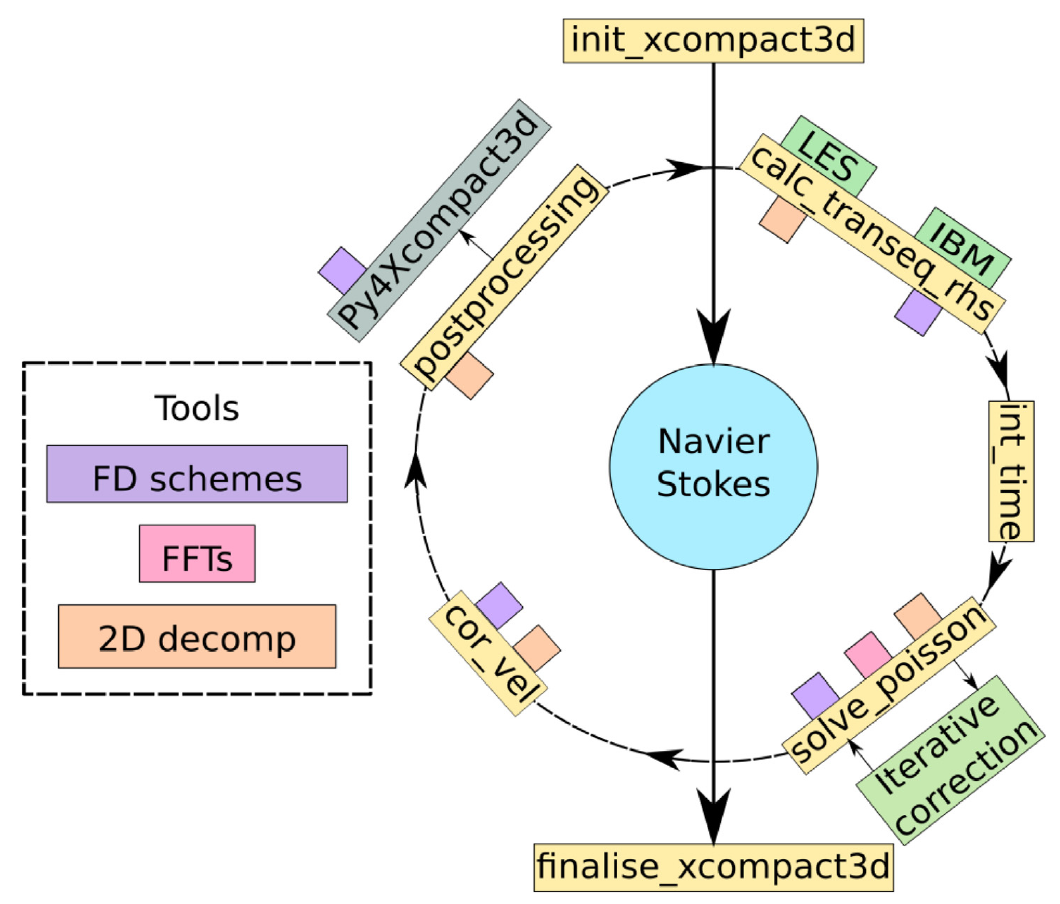
\includegraphics[width=0.49\textwidth]{figures/cap3/xc3d_architecture.png}
    	\label{fig:xc3d_archi}}  
    
    \subfloat[]{
    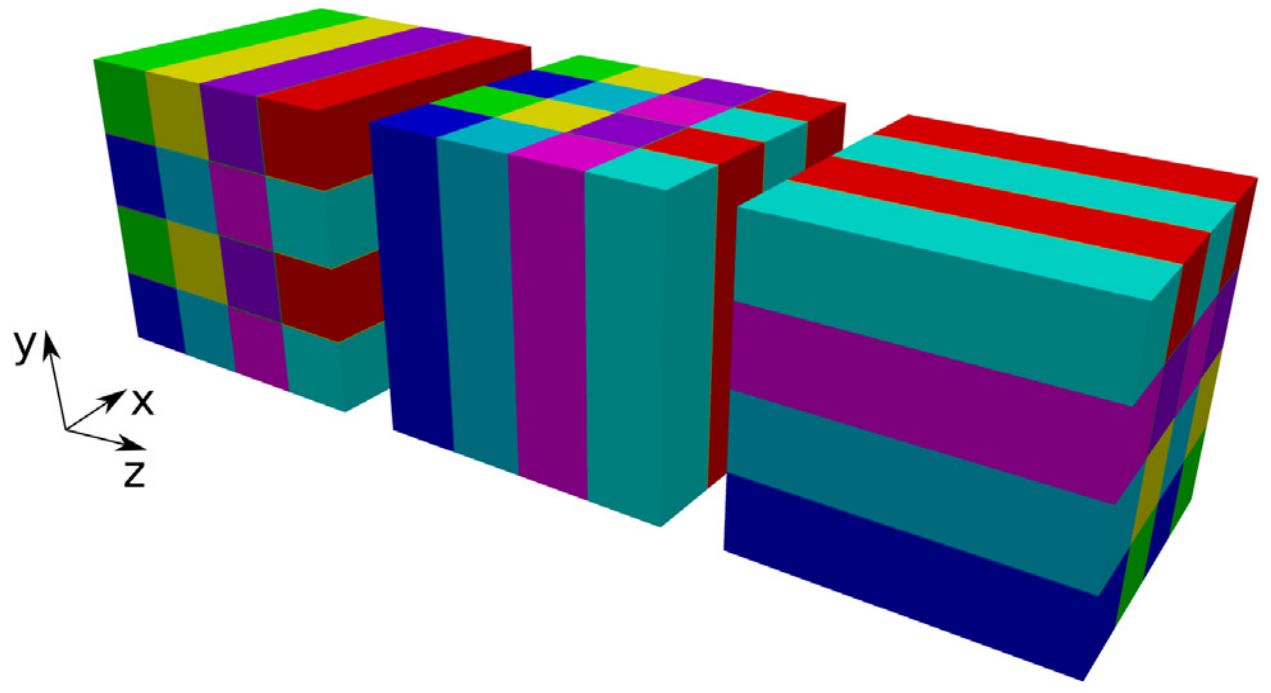
\includegraphics[width=0.49\textwidth]{figures/cap3/2d_decomp.png}
    	\label{fig:2d_decomp}}
 \caption{\textbf{(a)} Diagrama de la arquitectura de software de Xcompact3D. \textbf{(b)} Descomposición en lápices 2D utilizando 4 $\times$ 4 procesadores, representando los mismos en direcciones X, Y y Z respectivamente. Imágenes tomadas de \cite{bartholomew2020xcompact3d}.} 
 \label{fig:xc3d}
\end{figure}

El objetivo de las próximas subsecciones es ofrecer al lector una visión general de la lógica algorítmica de la herramienta numérica; se trata de un esquema conceptual a grandes rasgos, no de una descripción formal y rigurosa.

\subsection{Ecuaciones de gobierno}

Xcompact3D resuelve numéricamente las ecuaciones de Navier-Stokes para flujo incompresible junto con la ecuación de transporte de temperatura, acopladas entre sí mediante el término de fuerza boyante en la ecuación de momento. Las ecuaciones se expresan en forma adimensional en \ref{eq:sistem2} donde se omiten los superíndices ``*'' a fin de simplificar la notación. Obsérvese que si bien las ecuaciones están en consonancia con lo expuesto en el Capítulo \ref{cap:modelo}, no son exactamente las mismas. No obstante, estas ligeras diferencias no resultan relevantes en la explicación del método numérico.

\begin{equation}
\begin{aligned}
&\nabla \cdot \mathbf{u} = 0 \\
& \frac{\partial \mathbf{u}}{\partial t} = -\nabla \text{p} \underbrace{- (\mathbf{u} \cdot \nabla)\mathbf{u} + \frac{1}{\text{Re}} \nabla^2 \mathbf{u} + \mathbb{A} \hspace{0.5mm} \theta \hspace{0.5mm} \mathbf{e}_g + \mathbf{f} }_{\textbf{RHS}_{1}} \\
& \frac{\partial \theta}{\partial t} = \underbrace{- \mathbf{u} \cdot \nabla \theta + \frac{1}{\text{Re} \text{Pr}} \nabla^2 \theta + \mathbb{B} \hspace{0.5mm} u_x }_{\textbf{RHS}_2} \\
\end{aligned}
\label{eq:sistem2}
\end{equation}
En las ecuaciones precedentes: $\text{p}(\mathbf{x},t)$ es el campo de presiones; $\mathbf{u}(\mathbf{x},t)$ el campo de velocidades; $\theta(\mathbf{x},t)$ es el campo de temperatura; $\mathbf{x} = (x,y,z)$ es el vector de coordenadas y $t$ el tiempo; Re y Pr son los números adimensionales de Reynolds y Prandtl respectivamente; $\mathbb{A}$ y $\mathbb{B}$ son constantes que dependiendo de la forma adimensional considerada pueden ser diferentes, por ejemplo, tomando $\mathbb{A}=\text{Ri} / (\text{Re} \hspace{0.5mm} \text{Pr})$ y $\mathbb{B}=1$  se obtiene la forma adimensional de las ecuaciones \ref{eq:gob_system_adim}. La fuerza volumétrica $\mathbf{f}(\mathbf{x},t)$ es usado cuando se sumerge un cuerpo sólido dentro del dominio computacional (\textit{Immersed Boundary Method} \cite{peskin2002immersed}) o para otros usos según sea requerido.


\subsection{Esquemas de diferencias finitas de alto orden}

Las ventajas de los esquemas de alto orden para DNS/LES frente a los esquemas convencionales de bajo orden están plenamente reconocidas actualmente, especialmente por su capacidad de capturar con precisión un rango más amplio de escalas turbulentas para una resolución espacial dada. Los métodos espectrales estándar basados en representaciones de Fourier o de Chebyshev proporcionan soluciones muy precisas y eficientes de las ecuaciones de Navier-Stokes, aunque con severas restricciones en su aplicabilidad. Por su parte, los esquemas compactos de diferencias finitas de alto orden se aproximan a la precisión de los métodos espectrales y permiten mayor flexibilidad en la selección de condiciones de contorno (en XC3D es posible usar condiciones periódicas, de Dirichlet y de Neumann). Aunque los esquemas compactos son implícitos en el espacio, resultan muy competitivos en términos de eficiencia computacional. En particular, nuestras simulaciones emplean esquemas compactos de sexto orden para la discretización de los términos convectivo y difusivo.

\subsection{Avance temporal} \label{sec:time-ava}

El campo de flujo y el campo escalar se inicializan ya sea con una condición inicial (\texttt{init\_xcompact3d} en la Figura \ref{fig:xc3d_archi}) o cargando un archivo \textit{restart}. Las ecuaciones de Navier-Stokes se avanzan en el tiempo mediante un método de paso fraccionado (o proyección) implementado en tres etapas lógicas: (i) evaluación del lado derecho y \textit{predictor}, (ii) resolución de la ecuación de Poisson para la presión  e imposición de incompresibilidad y (iii) corrección de la velocidad y la temperatura.  En la Figura \ref{fig:xc3d_archi} se presenta una visión general de la arquitectura modular de \textit{Xcompact3D} \cite{bartholomew2020xcompact3d}. Las principales funcionalidades se separan en los modulos: \texttt{calc\_transeq\_rhs}, \texttt{int\_time}, \texttt{solve\_poisson}, \texttt{cor\_vel} y \texttt{postprocessing}. Los tres primeros corresponden a la resolución de las ecuaciones de gobierno, mientras que el último corresponde a la etapa de postprocesamiento de los datos obtenidos:


\begin{enumerate}
\item[\textbf{I}] \texttt{calc$\_$transeq$\_$rhs} $\rightarrow$ \texttt{int$\_$time}: predictor $\mathbf{u}^{\dagger \dagger}$ \\
Primero, se evalúan numéricamente los términos del lado derecho (\textbf{RHS}$_1$) de la ecuación de momento y se integran en el tiempo (una vez discretizados en el espacio) empleando, por ejemplo, esquemas de Runge-Kutta o Adams-Bashforth para obtener la velocidad intermedia $\mathbf{u}^{\dagger}$:

\begin{equation}
\frac{\mathbf{u}^{\dagger} - \mathbf{u}^k}{\Delta t} = \textbf{RHS}_1^k - c_k \nabla \widetilde{\text{p}}^k , 
\end{equation}
donde $c_k$ es un coeficiente conocido y $k$ el índice para los subpasos de tiempo \linebreak $k=1,...,n_k$; con $t_1=t_n$ y $t_{n_k}=t_{n+1}$ ($\Delta t = t_{n+1} - t_{n}$). La presión se expresa como su valor promediado en el tiempo en un subpaso dado ($c_k \Delta t$) indicado con una tilde $\widetilde{(\text{.})}$. Por conveniencia algebraica y para limpiar el lado derecho de la ecuación de Poisson de los pasos posteriores, puede definirse un campo intermedio $\mathbf{u}^{\dagger \dagger}$ que ``remueve'' la presión promedio usada en el predictor:

\begin{equation}
\frac{\mathbf{u}^{\dagger \dagger} - \mathbf{u}^{\dagger}}{\Delta t} = c_k \nabla \widetilde{\text{p}}^k  
\end{equation}
Con esta reordenación, $\mathbf{u}^{\dagger \dagger}$ sólo contiene los aportes no asociados a la presión previa:

\begin{equation}
\frac{\mathbf{u}^{\dagger \dagger} - \mathbf{u}^{k}}{\Delta t} = \textbf{RHS}_1^k \text{.}  
\end{equation}

\item[\textbf{II}] \texttt{solve\_poisson}: presión de proyección $\widetilde{p}^{k+1}$ \\
Se impone la incompresibilidad al final del paso:
	
\begin{equation}
\nabla \cdot \mathbf{u}^{k+1} = 0.
\label{eq:incomp}
\end{equation}
Tomando la divergencia de la corrección (véase ecuación \ref{eq:correccion}) y utilizando la ecuación \ref{eq:incomp}, se obtiene la ecuación de Poisson para la presión de proyección:

\begin{equation}
\nabla^2 \widetilde{\text{p}}^{k+1} = \frac{1}{c_k \Delta t} \nabla \cdot \mathbf{u}^{\dagger \dagger},
\end{equation}
donde $\widetilde{\text{p}}^{k+1}= \frac{1}{c_k \Delta t} \int^{t_{k+1}}_{t_k} \text{p} \hspace{0.5mm} dt$. 

Para la presión se aplican típicamente condiciones de borde de Neumann homogéneas (compatibles con la proyección). Por otro lado, las condiciones en la velocidad (por ejemplo, no deslizamiento) se aplican al predictor.

	\item[\textbf{III}]  \texttt{cor\_vel}: corrección solenoidal $\mathbf{u}^{k+1}$ \\
	Finalmente, se corrige la velocidad intermedia con el gradiente de la nueva presión para obtener
el campo solenoidal al final del paso de tiempo:

\begin{equation}
\frac{ \mathbf{u}^{k+1} - \mathbf{u}^{\dagger \dagger} }{\Delta t} = - c_k \nabla \widetilde{\text{p}}^{k+1} \text{.}
\label{eq:correccion}
\end{equation}

El término de la fuerza boyante no modifica la forma de la ecuación Poisson, sólo influye a través del predictor $\mathbf{u}^{\dagger \dagger}$ que genera. Adicionalmente, en el paso de tiempo actual $k$, se evalúa el lado derecho de la ecuación de transporte del escalar (\textbf{RHS}$_2$) empleando la velocidad del paso $k+1$, esto es:

\begin{equation}
\begin{aligned}
& \textbf{RHS}_2^k = - \mathbf{u}^{k+1} \cdot \nabla \theta^k + \frac{1}{\text{Re} \text{Pr}} \nabla^2 \theta^k + \mathbb{B} \hspace{0.5mm} u_x^{k+1}, \\
& \frac{\theta^{k+1} - \theta^{k}}{\Delta t} = \textbf{RHS}_2^k \text{.}
\end{aligned}
\end{equation}
Para la integración temporal de \textbf{RHS}$_2$ se emplea el mismo esquema utilizado en \textbf{RHS}$_1$.

\item[\textbf{IV}] \texttt{postprocessing} \\
Al final de cada paso de tiempo, el usuario puede decidir qué magnitudes almacenar y que cantidades calcular (magnitudes estadísticas de primer orden, segundo orden, etc).

\end{enumerate}

En particular, en este trabajo, para la integración temporal de los términos \textbf{RHS}$_{1,2}$ se emplea el esquema Adams-Bashforth de orden 3.



\subsection{\textit{Solver} espectral de Poisson}

Como se menciona en la Sección \ref{sec:time-ava}, Xcompact3D avanza las ecuaciones de gobierno mediante el método de paso fraccionario, formando una ecuación de Poisson para la presión al tomar la divergencia de la ecuación de momento. Una de las principales originalidades de Xcompact3D es que la ecuación de Poisson se resuelve en el espacio espectral usando el concepto de números de onda modificados \cite{lele1992compact}, para los cuales las operaciones en el espacio físico son estrictamente equivalentes a las del espacio espectral. Esta estrategia directa, que evita el uso de costosas técnicas iterativas, no es nueva para condiciones de contorno periódicas y/o de deslizamiento libre del campo de velocidades \cite{schumann1976direct}; asimismo, ha sido implementada y validada para condiciones de Dirichlet combinadas con esquemas de diferencias finitas de alto orden \cite{laizet2009high}.

\subsection{Biblioteca \textit{2D Decomp $\&$ FFT}}

Los esquemas de diferencias finitas y el \textit{solver} espectral de Poisson empleados por Xcompact3D se descomponen de forma natural en una serie de subproblemas unidimensionales. Por ello, resulta natural paralelizar el dominio computacional mediante una descomposición en “lápices”, como se ilustra en la Figura \ref{fig:2d_decomp}. Cada descomposición (en los ejes X, Y y Z, respectivamente) permite el cálculo independiente de derivadas, interpolaciones, etc. Las transposiciones globales para pasar de un lápiz a otro se realizan con comandos MPI. Más detalles sobre la estrategia de cómputo paralelo implementada en Xcompact3D pueden encontrarse en \cite{laizet2011incompact3d}.



\section{Orr-Somerfeld \textit{Mixed Convection} (OSMC)}

En el Capítulo \ref{cap:modelo}, empleando teoría de estabilidad lineal, considerando flujos laminares, y suponiendo las perturbaciones como ondas planas 3D (expresiones tipo \ref{eq:waves3d}) se arribó a un problema de autovalores y autofunciones generalizado, dado por la expresión \ref{eq:eigensistem-general}, con las condiciones de borde de la relación \ref{eq:eigensis-ci}. La herramienta numérica empleada para resolver este tipo de problemas es OSMC (por sus siglas, Orr-Somerfeld \textit{Mixed Convection}), desarrollada por Pablo Szuban como parte de su Proyecto Integrador de Ingeniería en el Instituto Balseiro \cite{szuban2023}. La herramienta numérica se implementó en lenguaje \textit{Python} utilizando las librerias \textit{NumPy} y \textit{SciPy}. La misma se encuentra disponible en GitHub: \href{https://github.com/Pato4184/OSMC-Repository}{OSMC-Repository}.

A continuación se dan los lineamientos detrás de la estrategia numérica utilizada. OSMC emplea el método numérico espectral conocido como ``Método de Colocación de la Matriz de Chebyshev'' \cite{moin2010fundamentals}. Esta estrategia busca transformar el problema de autovalores y autofunciones a uno de autovalores y autovectores. Los vectores solución son las amplitudes $\widehat{v_y}$, $\widehat{\varphi}$ y $\widehat{\eta}$ correspondientes a la frecuencia angular $\omega$ (autovalor asociado). Dado el sistema \ref{eq:eigensistem-general}, el flujo base laminar (Sección \ref{sec:fbase}) y las condiciones de borde asociadas, se discretiza la variable $y$ en el intervalo $\left[-1,1\right]$ en $N+1$ puntos de Chebyshev dados por la relación \ref{eq:cheb-points}. Lo siguiente es evaluar a las funciones involucradas en dichos puntos, por ejemplo, para una función arbitraria $\xi$ se tiene los puntos $\xi_j = \xi(y_j)$; luego, se construye un polinomio interpolante de Lagrange $\mathcal{L}$ para $\xi$ , de grado $\leq N$, tal que $\mathcal{L}(y_j) = \xi_j$.

\begin{equation}
y_j = \cos \left( \frac{j \hspace{0.5mm} \pi}{N} \right), \quad j=0,1,...,N 
\label{eq:cheb-points}
\end{equation}

De esta manera, los valores de la derivada de $\xi$ en los puntos $y_j$ son equivalentes a aquellos valores de la derivada del polinomio interpolante en los mismos puntos. Si $\xi$ se transforma a un vector\footnote{Es decir, los elementos $\xi_j$ del vector $\vec{\xi}$ son tales que $\xi_j = \xi(y_j)$.} $\vec{\xi}$, entonces, se puede demostrar \cite{moin2010fundamentals}, que la derivada de la función evaluada en los puntos de Chebyshev es $\vec{\xi^{\prime}} = \mathbb{D} \hspace{0.4mm} \vec{\xi}$ donde $\mathbb{D}$ es la Matriz de Colocación de Chebyshev de tamaño $(N+1) \times (N+1)$ \cite{trefethen}.

Si se tiene en cuenta que se necesita resolver un problema con condiciones de borde nulas (relaciones  \ref{eq:eigensis-ci}), es posible mostrar \cite{szuban2023}, que las primeras y últimas filas y columnas de la matriz $\mathbb{D}$ se pueden eliminar  de modo que resulta una matriz de $(N-1) \times (N-1)$ . Siguiendo este concepto, es posible obtener los operadores de derivada primera, segunda y cuarta, necesarios para la resolución del problema. Finalmente, al considerar todo lo explicitado, se obtiene un problema de autovalores y autovectores (generalizado) de matrices de tamaño  $3(N-1) \times 3(N-1)$ como se muestra en la expresión \ref{eq:eigensistem-matrix}. 

\begin{equation}
\begin{bmatrix}
A_{11} & A_{12} & \mathbb{O} \\[4pt]
A_{21} & A_{22} & A_{23} \\[4pt]
A_{31} & A_{32} & A_{33}
\end{bmatrix}
\,\begin{bmatrix}
\vec{\widehat{v_y} } \\[4pt]
\vec{\widehat{\varphi}} \\[4pt]
\vec{\widehat{\eta}}
\end{bmatrix}
\;=\; i \omega
\,\begin{bmatrix}
  B_1 & \mathbb{O} & \mathbb{O} \\[4pt]
    \mathbb{O} & \mathbb{I} & 0 \\[4pt]
    \mathbb{O} & \mathbb{O} & \mathbb{I}
\end{bmatrix}
\,\begin{bmatrix}
\vec{\widehat{v_y}} \\[4pt]
\vec{\widehat{\varphi}} \\[4pt]
\vec{\widehat{\eta}}
\end{bmatrix}
\label{eq:eigensistem-matrix}
\end{equation}

\begin{align*}
A_{11} &= \frac{1}{\text{Re}_b} \left[ \mathbb{D}^2 - k^2 \mathbb{I} \right]^2 - i \alpha \left( \mathtt{diag}(\vec{V_x}) ( \mathbb{D}^2 - k^2 \mathbb{I})  + \mathtt{diag}(\mathbb{D}^2 \vec{V_x}) \right) \hspace{2mm} ; \hspace{2mm} A_{12} = -\left[ i \alpha \frac{\text{Ra}}{\text{Re}_b} \mathbb{D} \right] \\ 
A_{21} &= \frac{i \alpha}{\text{Re}_b \hspace{1mm} \text{Pr} \hspace{1mm} k^2} \mathbb{D} + \mathtt{diag}(\mathbb{D}\vec{\Phi}) \hspace{2mm} ; \hspace{2mm} A_{22} = \frac{-1}{\text{Re}_b \hspace{1mm} \text{Pr} } \left[ \mathbb{D}^2 - k^2 \mathbb{I} \right] + i \alpha \hspace{0.4mm} \mathtt{diag}(\vec{V_x})  \hspace{2mm} ; \hspace{2mm} A_{23} = \frac{\beta}{\text{Re}_b \hspace{1mm} \text{Pr} \hspace{1mm} k^2} \mathbb{I} \\
A_{31} &= \beta \hspace{0.4mm} \mathtt{diag}(\mathbb{D} \vec{V_x}) \hspace{2mm} ; \hspace{2mm} A_{32} = - \beta \frac{\text{Ra}}{\text{Re}_b} \mathbb{I}   \hspace{2mm} ; \hspace{2mm} A_{33} = -\frac{1}{\text{Re}_b} \left[ \mathbb{D}^2 - k^2 \mathbb{I} \right] + i \alpha \hspace{0.4mm}  \mathtt{diag}(\vec{V_x}) \\
B_1    &= - \left[ \mathbb{D}^2 - k^2 \mathbb{I} \right] \hspace{2mm} ; \hspace{2mm} k^2 = \alpha^2 + \beta^2 \\
\end{align*}
Como puede observarse, las submatrices $A_{11}$, $A_{21}$, $A_{22}$, $A_{31}$ y $A_{33}$ tienen incorporado en su definición al operador $\mathtt{diag}$. El mismo transforma un vector $\vec{\xi}$, de tamaño $n \times 1$, en una matriz diagonal $n \times n$ cuyos elementos diagonales son los elementos de $\vec{\xi}$. Asimismo, $\mathbb{I}$ es la matriz identidad de tamaño $(N-1) \times (N-1)$ y $\mathbb{O}$ es la matriz nula de igual tamaño.



%\appendix
%\chapter{Ejemplo de ap\'{e}ndice: El problema de la medida}\label{C:ap1}
\chapterquote{Negociemos Don Inodoro}{Fernando de la R\'{u}a, 2001}
\chapterquote{Smartness runs in my family.  When I went to school I was so smart my
teacher was in my class for five years}{George Burns}
\graphicspath{{figs/}}
%%%%%%%%%%%%%%%%%%%%%%%%%%%%%%%%%%%%%%%%%%%%%%%%%%%%%%%%%%%%%%%%%%%%%%%%
El gran problema lo constituye el proceso de medici\'{o}n. En la f\'{\i}sica cl\'{a}sica, medir significa revelar o poner de manifiesto propiedades que estaban en el sistema desde antes de que midamos \cite{Philipp1982NCBSp75}.

En mec\'{a}nica cu\'{a}ntica el proceso de medici\'{o}n altera de forma incontrolada la evoluci\'{o}n del sistema. Constituye un error pensar dentro del marco de la f\'{\i}sica cu\'{a}ntica que medir es revelar propiedades que estaban en el sistema con anterioridad. La informaci\'{o}n que nos proporciona la funci\'{o}n de onda es la distribuci\'{o}n de probabilidades, con la cual se podr\'{a} medir tal valor de tal cantidad. Cuando medimos ponemos en marcha un proceso que es indeterminable a priori, lo que algunos denominan azar, ya que habr\'{a} distintas probabilidades de medir distintos resultados. Esta idea fue y es a\'{u}n objeto de controversias y disputas entre los f\'{\i}sicos, fil\'{o}sofos y epistem\'{o}logos. Uno de los grandes objetores de esta interpretaci\'{o}n fue Albert Einstein, quien a prop\'{o}sito de esta idea dijo su famosa frase "Dios no juega a los dados".

Independientemente de los problemas de interpretaci\'{o}n, la mec\'{a}nica cu\'{a}ntica ha podido explicar esencialmente todo el mundo microsc\'{o}pico y ha hecho predicciones que han sido probadas experimentalmente de forma exitosa, por lo que es una teor\'{\i}a un\'{a}nimemente aceptada.

\begin{figure}[ht]
\centering{}
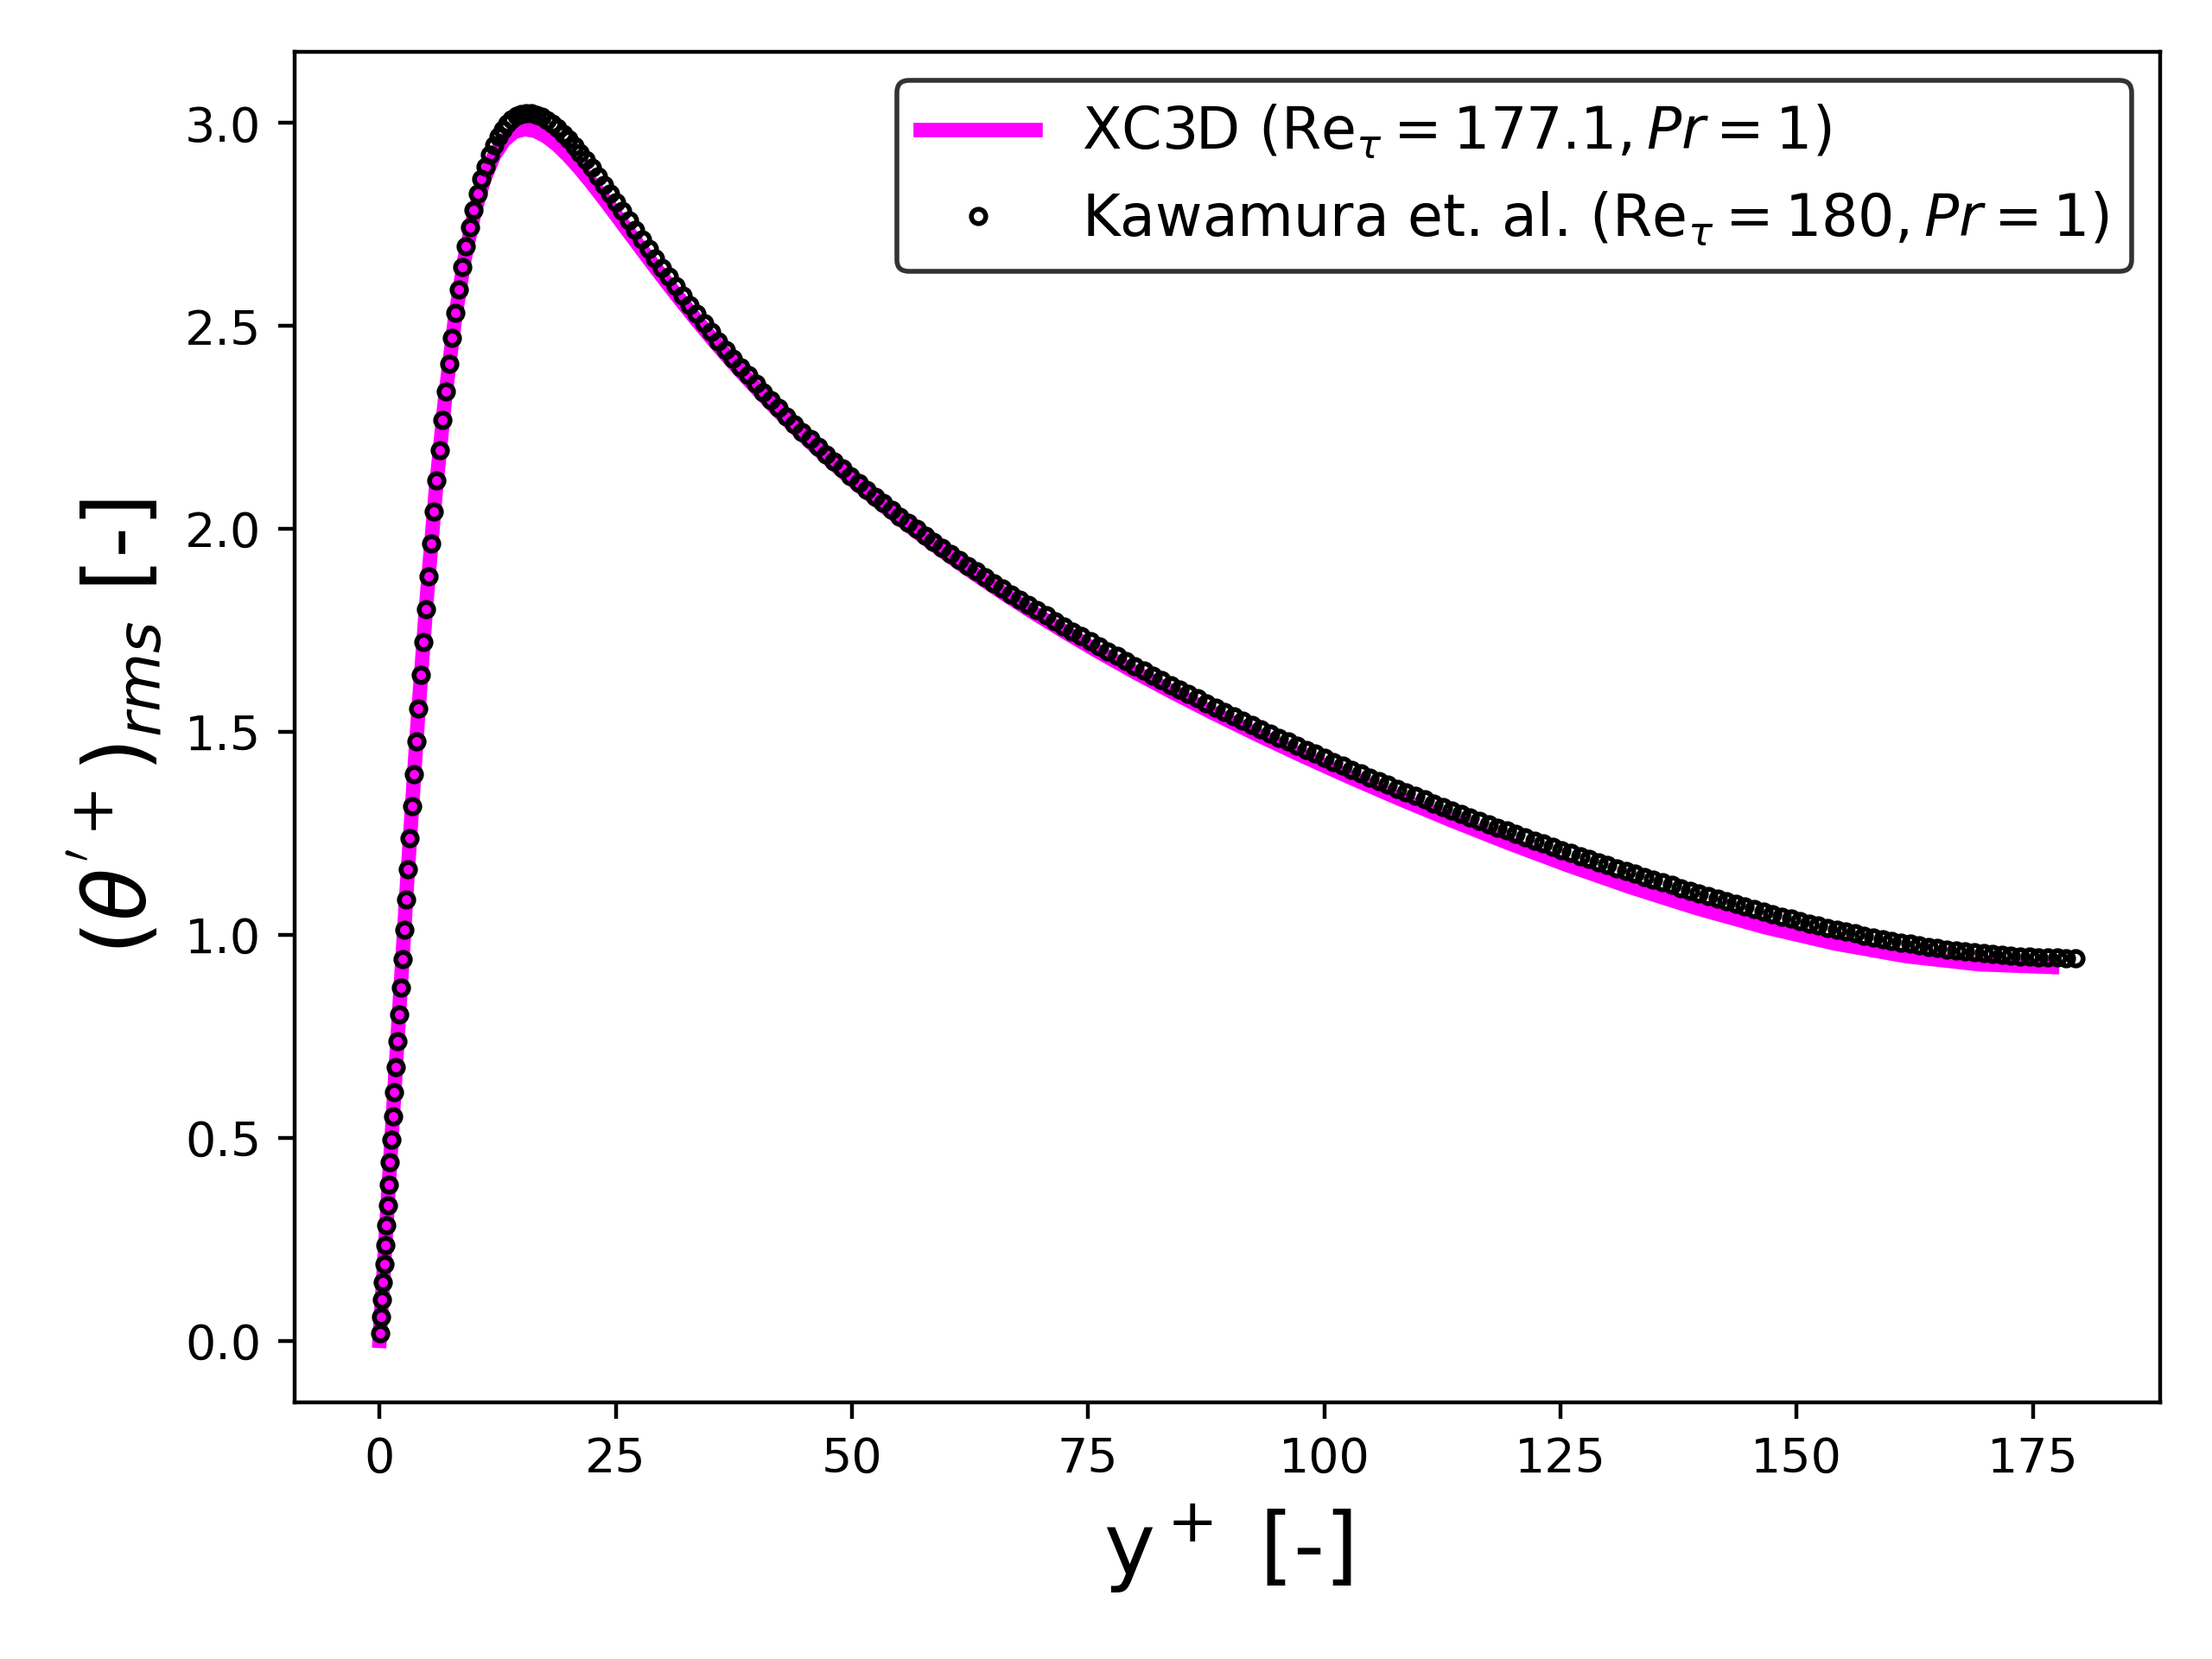
\includegraphics[width=\imsize]{results/Ret180_Pr1_theta_rms.png}
\caption{CAPTION}
\label{fig:apend}  
\end{figure}



%%% Local Variables: 
%%% mode: latex
%%% TeX-master: "template"
%%% End: 



\bibliographystyle{apalike}
\bibliography{references}
\addcontentsline{toc}{chapter}{Bibliografía}

\begin{postliminary}

%\begin{seccion}{Publicaciones asociadas}
%  \begin{enumerate}
%  \item Mi primer aviso en la revista \textbf{ABC}, 1996
%  \item Mi segunda publicaci\'{o}n en la revista \textbf{ABC}, 1997
%  \end{enumerate}
%\end{seccion}

\begin{seccion}{Agradecimientos}
\chapterquote{Oh if I get lost, I know I can return ... \\
 There's a drink awaiting me at the tavern ...}{Lilith Max}
 
A todos los que se lo merecen, por merecerlo
\end{seccion}

\end{postliminary}

\end{document}

